%  KeySpark manuscript prepared for MDPI Sensors.
%  Apart from tables/manual_related.tex and figures/dataflow.tex, which are written
%  by hand, the fragments in tables/ and figures/ are outputs of the scripts in
%  ../paper/scripts, with wording adapted for the journal.
\documentclass[sensors,article,submit,pdftex,oneauthor]{Definitions/mdpi}

\usepackage{pgfplots}
\pgfplotsset{compat=1.18}
\usetikzlibrary{positioning,arrows.meta,fit,patterns}
\usepackage{etoolbox}
% The class pulls the first Highlights line 6pt up into the heading; give it room instead.
\patchcmd{\abstractkeywords}{\textbf{Highlights\vspace{-6pt}\\}}{\textbf{Highlights}\\[3pt]}{}{\PackageWarning{main}{Highlights patch failed}}

\newcommand{\TODO}[1]{\textcolor{red}{[TODO: #1]}}

%=================================================================
\firstpage{1}
\makeatletter
\setcounter{page}{\@firstpage}
\makeatother
\pubvolume{1}
\issuenum{1}
\articlenumber{0}
\pubyear{2026}
\copyrightyear{2026}
\datereceived{ }
\daterevised{ }
\dateaccepted{ }
\datepublished{ }

%=================================================================
\Title{Detecting Input Automation in Keyboard and Mouse Event Streams: A Streaming Pipeline with Content-Free Features and a Leakage-Aware Evaluation}

% ORCID (optional): define \newcommand{\orcidauthorA}{0000-...} and add \orcidA{} after the name.
\Author{Murat Emirhan Aykut}

\AuthorNames{Murat Emirhan Aykut}

\address{%
Artificial Intelligence Department, Bah\c{c}e\c{s}ehir University, 34353 Istanbul, T\"urkiye; muratemirhan.aykut@bahcesehir.edu.tr}

\corres{Correspondence: muratemirhan.aykut@bahcesehir.edu.tr}

%=================================================================
\abstract{Keyboards and pointing devices are human interface device sensors whose event timing can reveal automated input, whatever is typed. This study asks whether input automation can be detected continuously from content-free stream features, and what holding out sessions and automation kinds reveals. KeySpark processes host input with Apache Kafka and Spark in a Lambda architecture; engine kills and broker restarts lost nothing, expired retention lost events, and re-sent events were duplicated. On 2.80 million events of one user and 16 generated sessions of four kinds, a random forest on seven one-minute window features achieves an $F_1$ of 0.988 (95\% interval 0.979 to 0.996) with every kind in training. Held-out kinds stay almost perfectly ranked (area under the curve 0.969 to 1.000), but the fixed threshold fails (mean $F_1$ 0.459). For this forest, seen-kind thresholds do not help, whereas a 1\% genuine false-positive budget raises the mean $F_1$ to 0.782; over 40 partitions and five generator seeds with 2 to 32 sessions per kind, held-out recall stays at 0.75 to 0.83, against at most 0.56. A published feature set reaches 0.958, partly through generator artefacts. No real tool was captured; generated sessions at default tool settings were abstained on or missed.}

\keyword{keystroke dynamics; mouse dynamics; input automation; behavioural biometrics; bot detection; event-based sensing; stream processing; Lambda architecture; human--computer interaction}

% The class tests \@addhighlights for emptiness and then calls \addhighlights,
% expecting the .tex to redefine it with the itemized content.
\makeatletter
\gdef\@addhighlights{yes}
\makeatother
\renewcommand{\addhighlights}{%
\textbf{What are the main findings?}
\begin{itemize}
\item A random forest on seven content-free features separates one user's input from four kinds of generated automation ($F_1$ 0.988 when every kind appears in training and testing), and the separation holds when both classes are restricted to the same event types.
\item For this random forest, automation kinds held out of training stay almost perfectly ranked, but the threshold learned on the other kinds does not transfer, even when tuned on them; a threshold set from the genuine score distribution alone raises held-out recall well above the fixed and seen-kind thresholds at every synthetic-class size from 2 to 32 sessions per kind. A richer published feature set scores higher on unseen kinds, partly through structural artefacts of the generator.
\end{itemize}
\textbf{What are the implications of the main findings?}
\begin{itemize}
\item In this study, holding out whole automation kinds changed the conclusions, whereas holding out sessions instead of windows changed the $F_1$ score only slightly; detectors trained on synthetic automation should therefore be evaluated on held-out kinds.
\item This one-minute detector abstains on, or misses, generated sessions that follow keep-active tools' default settings, so slow tools need longer windows, capture-level signals, or key-class features.
\end{itemize}}

%=================================================================
\begin{document}

%=================================================================
\section{Introduction}
\label{sec:intro}

Keyboards and pointing devices act as human interface device (HID) sensors. Each reports discrete state transitions, such as key presses and releases or button and wheel changes, and relative pointer displacement at irregular, event-driven times. During ordinary work these sensors emit an unbounded stream of low-level events that arrives in bursts separated by idle periods. Keystroke and mouse dynamics derived from this stream are an established behavioural signal for authentication and identification~\cite{monrose2000keystroke, teh2013survey, kasprowski2022keystroke, wycislik2024keystroke, lis2023siamese, subash2026adaptability}, for affective and cognitive states~\cite{epp2011identifying, kolakowska2021opinions, acien2022fatigue}, and for separating human from automated input~\cite{gianvecchio2009botcraft, acien2022becaptcha}. Sensors has published several such studies as behavioural sensing~\cite{wang2022siurua, kasprowski2022keystroke, wycislik2024keystroke, lis2023siamese}.

Most of these studies analyse recorded sessions offline, but detecting automation on a working computer is a different task. The stream must be processed continuously, the features must not depend on what is typed, and order-dependent quantities such as session boundaries must stay correct while events arrive late or the host sleeps. A detector built for that setting also has to be evaluated differently. One-minute windows from the same session are strongly correlated, and the automation class is usually synthetic. As a result, a hold-out drawn over windows can measure recall of a session or a generator the model has already seen rather than generalisation.

This study therefore asks two linked questions. First, can input automation be detected continuously from content-free features of a host's keyboard and mouse event stream? Second, what does an evaluation that holds out whole sessions and whole tool families, here called automation kinds, reveal about a detector trained against synthetic automation? The first working hypothesis (H1) is that one user's input is more irregular than generated automation modelled on keep-active tools; it is tested by the $F_1$ score of a detector evaluated on held-out sessions. The second (H2) is that a detector trained on some automation kinds generalises to a kind absent from training; it is tested by the leave-one-kind-out $F_1$ score at the detector's operating points. No numeric criterion was fixed in advance; H1 is judged against the rule and learner baselines of Section~\ref{sec:features-models}, and H2 by how close the held-out kinds come to the $F_1$ score of the kind-stratified design.

To answer them, KeySpark ingests input events through a durable and replayable Kafka log, computes per-minute metrics with event-time windows, watermarking, and checkpointed sinks, and computes session-level and order-dependent analytics in a batch layer. Each one-minute window is classified as human or automated from seven cross-modal shape features. The detection study is a longitudinal single-subject case study: 22 days and 242 sessions of the author's own input, against four kinds of synthetic automation.

The main contributions of this paper are as follows:
\begin{itemize}
\item A streaming pipeline for keyboard and mouse events whose analytics and detector features are content-free, with order-dependent metrics computed in a batch layer. Its throughput against micro-batch size is characterised on 2.96 million events, and its latency from the Kafka topic to the per-minute output and its recovery from injected faults are measured on the deployed path.
\item A leakage-aware evaluation protocol for window-level automation detection. It combines session-wise and kind-stratified hold-outs with session-level confidence intervals, leave-one-kind-out generalisation, an event-type check, a test at the default settings of real tools, and a day-level decision analysis checked on later days.
\item Evidence that a random forest trained on synthetic automation ranks unseen automation kinds almost perfectly yet fails at its fixed threshold. A threshold set from the genuine score distribution alone raises held-out recall well above the fixed and seen-kind thresholds at every synthetic-class size from 2 to 32 sessions per kind, at a false-positive rate near 1\%; with one session per kind a seen-kind threshold does as well. For logistic regression it bounds the false-positive rate but does not recover $F_1$. A comparison with a published feature set shows how far cross-kind scores reflect artefacts of the generator.
\item An open, content-free per-window dataset and code that reproduce the session-wise, kind-stratified, leave-one-kind-out, operating-point, and day-level results.
\end{itemize}

Section~\ref{sec:related} reviews related work, and Section~\ref{sec:methods} describes the data, the pipeline, the detector, and the evaluation protocol. Section~\ref{sec:results} presents the results, Section~\ref{sec:discussion} discusses them together with their limitations, and Section~\ref{sec:conclusions} concludes.

%=================================================================
\section{Related Work}
\label{sec:related}

This study draws on stream processing of sensor and interaction data, keyboard and mouse dynamics as a behavioural signal, and the detection of input automation.

\subsection{Stream Processing of Sensor and Interaction Data}
Apache Kafka introduced the partitioned, replayable commit log as a substrate for decoupling event producers from consumers~\cite{kreps2011kafka}, and it serves as the ingestion bus of KeySpark. Apache Spark's resilient distributed datasets provide a fault-tolerant in-memory engine~\cite{zaharia2012rdd}, and its Structured Streaming application programming interface (API) models an unbounded stream as a continuously growing table~\cite{armbrust2018structured}. The Lambda architecture pairs a low-latency speed layer with a batch layer that acts as the source of truth~\cite{marz2015bigdata}.

Several studies in this journal apply these components to sensor data. Demirezen and Navruz~\cite{demirezen2023lambda} tested the accuracy of a Lambda-architecture system on air and ground surveillance data. They injected repeated and delayed data and compared served results with an independent ground truth, the approach adopted for the fault tests here. Khattach et al.~\cite{khattach2025iot} combined Kafka-based ingestion with Spark extraction, transformation, and loading for Internet of Things analytics. Pal et al.~\cite{pal2023clickstream} ingested a browser clickstream through Apache Storm, Kafka, and Cassandra within a Lambda architecture, a close structural analogue that operates on web clicks rather than raw input events. Personal-productivity tools such as TimeAware~\cite{kim2016timeaware}, by contrast, ingest data periodically and track application-usage time. KeySpark is a single-machine instantiation of the Lambda architecture over raw input events, in which order-dependent metrics are computed in the batch layer.

\subsection{Keyboard and Mouse Dynamics}
Keystroke dynamics describe typing through timing features such as key hold and flight times and form an established behavioural biometric~\cite{monrose2000keystroke, teh2013survey}; Killourhy and Maxion~\cite{killourhy2009comparing} provided a widely used benchmark for comparing detectors. Mouse dynamics describe pointer movement through speed, direction, and action features, and have been used for authentication since Ahmed and Traore~\cite{ahmed2007mouse} and Shen et al.~\cite{shen2013mouse}. Kasprowski et al.~\cite{kasprowski2022keystroke} studied how network architecture and hyperparameters affect keystroke-based identification, and Wyci\'slik et al.~\cite{wycislik2024keystroke} improved identification on open datasets with deep learning. Lis et al.~\cite{lis2023siamese} authenticated users from partial-password typing without recording which keys were pressed, the same content-free principle followed here. Wang et al.~\cite{wang2022siurua} fused keystroke and mouse features computed over time windows for authentication across usage scenes; their feature set is used as a comparison in Section~\ref{sec:features-models}. Keystroke patterns have also been related to emotional states~\cite{epp2011identifying}, the polarity of written opinions~\cite{kolakowska2021opinions}, mental fatigue~\cite{acien2022fatigue}, and office-worker productivity together with other sensors~\cite{awada2023productivity}. Subash et al.~\cite{subash2026adaptability} surveyed how keystroke and mouse biometrics adapt to changing behaviour. KeySpark reuses features of this kind to ask whether a minute of input was produced by a person at all, not who produced it.

\subsection{Detection of Input Automation}
Distinguishing human from automated input is a long-standing security problem. Gianvecchio et al.~\cite{gianvecchio2009botcraft} detected game bots passively from the input stream rather than through an interactive challenge, the approach adopted here. Chu et al.~\cite{chu2012cyborg} separated human, bot, and mixed accounts on Twitter from behavioural features. Other studies detected web bots from keystroke dynamics against diffusion-synthesised keystrokes~\cite{see2024webbots}, from mouse movements rendered as images~\cite{niu2023visual, niu2024lightweight}, from both modalities in web sessions~\cite{modi2026comparison}, from web logs combined with mouse behaviour~\cite{iliou2021webbots}, and from browsing behaviour at scale~\cite{kadel2024botracle}. Wilczek et al.~\cite{wilczek2026intruder} detected impersonation from web-server logs, and, closest to the present setting, Acien et al.~\cite{acien2022becaptcha} separated human from bot mouse trajectories while training partly on synthetic trajectories.

Table~\ref{tab:related} compares the data provenance of these studies with the present one. They differ in data source, population, the origin of the automation class, and the decision unit, so their scores cannot be compared directly with those reported here. For this reason, Section~\ref{sec:features-models} evaluates an established feature set and a one-class detector on the present data instead. KeySpark differs from these studies in three respects: it scores a combined keyboard and mouse stream continuously on the host, it uses only content-free features, and its automation class is entirely synthetic. Section~\ref{sec:training} compares that class with the documented behaviour of real keep-active tools.

% manual table -- authored by hand; provenance cells taken from the cited
% works' own published descriptions (abstracts and released benchmarks),
% consulted 2026-08
\begin{table}[H]
\caption{Data provenance of input-behaviour bot-detection work published from
2022 on, against the present study. Scores are deliberately omitted; see the text.}
\label{tab:related}
\centering
\footnotesize
\begin{adjustwidth}{-\extralength}{0cm}\resizebox{\linewidth}{!}{\begin{tabular}{lllll}
\toprule
Work & Data source & Subjects & Automation-class origin & Decision unit \\
\midrule
See et al.~\cite{see2024webbots} & web keystroke dynamics & not stated & diffusion-model synthetic keystrokes & keystroke sequence \\
Niu et al.~\cite{niu2023visual} & mouse movements, login task & 150 & authors' scripted bots & mouse-movement image \\
Niu et al.~\cite{niu2024lightweight} & mouse movements, login task & 150 & authors' scripted bots & mouse-movement image \\
Modi et al.~\cite{modi2026comparison} & web-session keystroke and mouse data & not stated & not stated & web request \\
Acien et al.~\cite{acien2022becaptcha} & mouse trajectories (15{,}000) & 58 & function-based and GAN synthetic (part) & mouse trajectory \\
Kadel et al.~\cite{kadel2024botracle} & e-commerce traffic, $\sim$40M visits/mo & site visitors & heuristic (cloud IPs, agent/timing) & request and session \\
This paper & self-collected keyboard and mouse events & 1 & synthetic generator, entirely & one-minute window \\
\bottomrule
\end{tabular}}\end{adjustwidth}
\par\vspace{2pt}\noindent\footnotesize Cells restate what each cited work reports about its own
data in its published abstract or released benchmark, consulted in August
2026; ``not stated'' marks details the freely accessible sources do not give.
Earlier work cited in the text is not listed.
IP, Internet Protocol; GAN, generative adversarial network.
\end{table}


%=================================================================
\section{Materials and Methods}
\label{sec:methods}

This section describes the data, the pipeline that captures and processes them, the detector, and the evaluation protocol.

\subsection{Data Acquisition}
\label{sec:dataset}

The dataset was collected from a single user, the author, during ordinary work on their own computer between 21 May and 18 June 2026.

\subsubsection{Capture, Privacy, and Ethics}
\label{sec:capture}
A native capture agent built on the pynput library~\cite{pynput} records the keyboard and mouse events of the host and emits each event as a JavaScript Object Notation (JSON) record. Each key event carries a key identifier, which is the character for printable keys and a symbolic name for special keys. This identifier bounds every privacy claim in this paper, because it is retained beside its timestamp, so that ordering the \texttt{key\_down} events by time reconstructs the typed text. The measured archive is thus a plaintext corpus, held locally on the capture host and never transmitted or released. Mouse-move events are throttled to a minimum interval of 20\,ms, about 50 events per second, to bound data volume, while clicks and scrolls are never throttled.

Everything computed from the archive is content-free. The per-minute metrics, the session and baseline analytics, the seven features of Section~\ref{sec:method}, and the dashboard use the key identifier only through counts, timings, and the number of distinct keys within a minute. None of them retains or exposes which key was pressed. A transform that replaces the identifier with a coarse key class and a minute-rotating keyed token is implemented and unit-tested in the released code. Within one minute the token maps each key consistently, so a transformed record is pseudonymised rather than anonymised, and how much typed text could be recovered from it was not assessed. The measured deployment stored raw identifiers, but Section~\ref{sec:features-models} shows that the classification results are essentially unchanged when computed through the transform.

Only the author's input was captured, but because the archive is plaintext, it may contain text typed about or to other people; it is therefore held offline, never transmitted, and will be deleted after publication. The motivating application is in practice a workplace-monitoring capability, as in other keyboard and mouse logging studies~\cite{awada2023productivity}, and the day-level policy of Section~\ref{sec:method} flags whole working days. The false-alarm rates of Section~\ref{sec:daypolicy} are measured on one subject against a synthetic adversary and do not support using such a flag as evidence about a worker.

\subsubsection{Event Schema}
Events are parsed into an explicit ten-field typed schema and stored in the columnar Parquet format. The fields are the event \texttt{type} (one of \texttt{key\_down}, \texttt{key\_up}, \texttt{move}, \texttt{click}, or \texttt{scroll}), the key identifier, the pointer coordinates, deltas, and button state (populated only for pointer events), the user identifier, and the event timestamp.

\subsubsection{Corpus Composition}
Table~\ref{tab:dataset} summarises the genuine corpus after the data freeze. During development, three seeded demonstration days and a test user were injected to exercise the classifier. They are excluded from the genuine class, as in the released code, and reused in Section~\ref{sec:daypolicy} as automation days. These days are distinguishable by objective criteria rather than by inspection of results. They contain no \texttt{key\_up} and no \texttt{scroll} events and only 12 distinct keys, against 86 to 119 on genuine days, and their most frequent keys, \texttt{scroll\_lock} and \texttt{f13}, are those emitted by keep-awake utilities. The genuine subset holds 2,804,614 events, and the complete archive of 2,962,308 events is what the deployed pipeline processes and the throughput benchmarks read. Although mouse movement is throttled at capture, \texttt{scroll} events are not and form the largest event type, at 41.9\,\% of the genuine archive. Figure~\ref{fig:day} shows one day of the corpus.

% generated by Paperino/scripts/make_tables.py -- do not edit by hand
\begin{table}[H]
\caption{Genuine corpus after the data freeze.}
\label{tab:dataset}
\centering
\begin{tabular}{lr}
\toprule
Quantity & Value \\
\midrule
Events & 2,804,614 \\
Active days & 22 \\
Collection span & 2026-05-21 to 2026-06-18 \\
Sessions (5-min idle gap) & 242 \\
Active time (hours) & 65.8 \\
Median session (minutes) & 9.8 \\
\midrule One-minute windows & 3,729 \\
\quad scored ($\geq 5$ events) & 3,649 \\
\quad abstained ($< 5$ events) & 80 \\
\midrule \texttt{scroll} events & 1,174,379 (41.9\%) \\
\texttt{move} events & 1,124,156 (40.1\%) \\
\texttt{key\_down} events & 227,895 (8.1\%) \\
\texttt{key\_up} events & 222,578 (7.9\%) \\
\texttt{click} events & 55,606 (2.0\%) \\
\midrule Distinct keys & 130 \\
Word boundaries (space) & 27,590 \\
Corrections (backspace/delete) & 16,277 (7.1\%) \\
\bottomrule
\end{tabular}
\\[2pt] \footnotesize Seeded demonstration days and the test user are excluded, as in the released code.
\end{table}


% generated by Paperino/scripts/dayplot.py -- do not edit by hand
\begin{figure}[H]
\centering
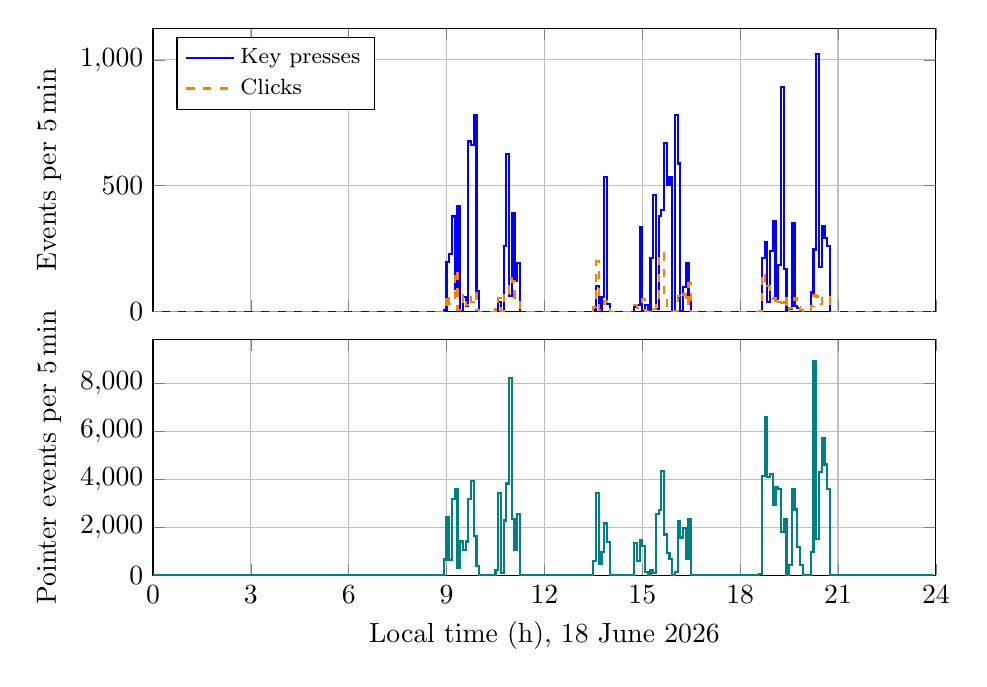
\begin{tikzpicture}
\begin{axis}[
  name=top, width=0.82\linewidth, height=3.6cm, scale only axis,
  xmin=0, xmax=24, xtick={0,3,6,9,12,15,18,21,24}, xticklabels={},
  ymin=0, ylabel={Events per 5\,min}, grid=major,
  legend pos=north west, legend cell align=left, legend style={font=\footnotesize},
]
\addplot[const plot, thick, color=blue] coordinates {(0.000,0) (0.083,0) (0.167,0) (0.250,0) (0.333,0) (0.417,0) (0.500,0) (0.583,0) (0.667,0) (0.750,0) (0.833,0) (0.917,0) (1.000,0) (1.083,0) (1.167,0) (1.250,0) (1.333,0) (1.417,0) (1.500,0) (1.583,0) (1.667,0) (1.750,0) (1.833,0) (1.917,0) (2.000,0) (2.083,0) (2.167,0) (2.250,0) (2.333,0) (2.417,0) (2.500,0) (2.583,0) (2.667,0) (2.750,0) (2.833,0) (2.917,0) (3.000,0) (3.083,0) (3.167,0) (3.250,0) (3.333,0) (3.417,0) (3.500,0) (3.583,0) (3.667,0) (3.750,0) (3.833,0) (3.917,0) (4.000,0) (4.083,0) (4.167,0) (4.250,0) (4.333,0) (4.417,0) (4.500,0) (4.583,0) (4.667,0) (4.750,0) (4.833,0) (4.917,0) (5.000,0) (5.083,0) (5.167,0) (5.250,0) (5.333,0) (5.417,0) (5.500,0) (5.583,0) (5.667,0) (5.750,0) (5.833,0) (5.917,0) (6.000,0) (6.083,0) (6.167,0) (6.250,0) (6.333,0) (6.417,0) (6.500,0) (6.583,0) (6.667,0) (6.750,0) (6.833,0) (6.917,0) (7.000,0) (7.083,0) (7.167,0) (7.250,0) (7.333,0) (7.417,0) (7.500,0) (7.583,0) (7.667,0) (7.750,0) (7.833,0) (7.917,0) (8.000,0) (8.083,0) (8.167,0) (8.250,0) (8.333,0) (8.417,0) (8.500,0) (8.583,0) (8.667,0) (8.750,0) (8.833,0) (8.917,6) (9.000,197) (9.083,230) (9.167,378) (9.250,91) (9.333,420) (9.417,4) (9.500,59) (9.583,24) (9.667,676) (9.750,661) (9.833,782) (9.917,81) (10.000,0) (10.083,0) (10.167,0) (10.250,0) (10.333,0) (10.417,0) (10.500,0) (10.583,37) (10.667,0) (10.750,260) (10.833,626) (10.917,61) (11.000,391) (11.083,121) (11.167,192) (11.250,0) (11.333,0) (11.417,0) (11.500,0) (11.583,0) (11.667,0) (11.750,0) (11.833,0) (11.917,0) (12.000,0) (12.083,0) (12.167,0) (12.250,0) (12.333,0) (12.417,0) (12.500,0) (12.583,0) (12.667,0) (12.750,0) (12.833,0) (12.917,0) (13.000,0) (13.083,0) (13.167,0) (13.250,0) (13.333,0) (13.417,0) (13.500,8) (13.583,102) (13.667,7) (13.750,57) (13.833,534) (13.917,31) (14.000,0) (14.083,0) (14.167,0) (14.250,0) (14.333,0) (14.417,0) (14.500,0) (14.583,0) (14.667,0) (14.750,20) (14.833,27) (14.917,337) (15.000,4) (15.083,28) (15.167,0) (15.250,214) (15.333,462) (15.417,10) (15.500,379) (15.583,403) (15.667,670) (15.750,505) (15.833,533) (15.917,0) (16.000,780) (16.083,588) (16.167,4) (16.250,97) (16.333,192) (16.417,45) (16.500,0) (16.583,0) (16.667,0) (16.750,0) (16.833,0) (16.917,0) (17.000,0) (17.083,0) (17.167,0) (17.250,0) (17.333,0) (17.417,0) (17.500,0) (17.583,0) (17.667,0) (17.750,0) (17.833,0) (17.917,0) (18.000,0) (18.083,0) (18.167,0) (18.250,0) (18.333,0) (18.417,0) (18.500,0) (18.583,0) (18.667,212) (18.750,277) (18.833,37) (18.917,241) (19.000,358) (19.083,52) (19.167,186) (19.250,892) (19.333,170) (19.417,8) (19.500,12) (19.583,352) (19.667,22) (19.750,16) (19.833,0) (19.917,0) (20.000,0) (20.083,0) (20.167,76) (20.250,247) (20.333,1023) (20.417,178) (20.500,339) (20.583,292) (20.667,262) (20.750,0) (20.833,0) (20.917,0) (21.000,0) (21.083,0) (21.167,0) (21.250,0) (21.333,0) (21.417,0) (21.500,0) (21.583,0) (21.667,0) (21.750,0) (21.833,0) (21.917,0) (22.000,0) (22.083,0) (22.167,0) (22.250,0) (22.333,0) (22.417,0) (22.500,0) (22.583,0) (22.667,0) (22.750,0) (22.833,0) (22.917,0) (23.000,0) (23.083,0) (23.167,0) (23.250,0) (23.333,0) (23.417,0) (23.500,0) (23.583,0) (23.667,0) (23.750,0) (23.833,0) (23.917,0)};
\addlegendentry{Key presses}
\addplot[const plot, thick, dashed, color=orange] coordinates {(0.000,0) (0.083,0) (0.167,0) (0.250,0) (0.333,0) (0.417,0) (0.500,0) (0.583,0) (0.667,0) (0.750,0) (0.833,0) (0.917,0) (1.000,0) (1.083,0) (1.167,0) (1.250,0) (1.333,0) (1.417,0) (1.500,0) (1.583,0) (1.667,0) (1.750,0) (1.833,0) (1.917,0) (2.000,0) (2.083,0) (2.167,0) (2.250,0) (2.333,0) (2.417,0) (2.500,0) (2.583,0) (2.667,0) (2.750,0) (2.833,0) (2.917,0) (3.000,0) (3.083,0) (3.167,0) (3.250,0) (3.333,0) (3.417,0) (3.500,0) (3.583,0) (3.667,0) (3.750,0) (3.833,0) (3.917,0) (4.000,0) (4.083,0) (4.167,0) (4.250,0) (4.333,0) (4.417,0) (4.500,0) (4.583,0) (4.667,0) (4.750,0) (4.833,0) (4.917,0) (5.000,0) (5.083,0) (5.167,0) (5.250,0) (5.333,0) (5.417,0) (5.500,0) (5.583,0) (5.667,0) (5.750,0) (5.833,0) (5.917,0) (6.000,0) (6.083,0) (6.167,0) (6.250,0) (6.333,0) (6.417,0) (6.500,0) (6.583,0) (6.667,0) (6.750,0) (6.833,0) (6.917,0) (7.000,0) (7.083,0) (7.167,0) (7.250,0) (7.333,0) (7.417,0) (7.500,0) (7.583,0) (7.667,0) (7.750,0) (7.833,0) (7.917,0) (8.000,0) (8.083,0) (8.167,0) (8.250,0) (8.333,0) (8.417,0) (8.500,0) (8.583,0) (8.667,0) (8.750,0) (8.833,0) (8.917,16) (9.000,68) (9.083,32) (9.167,32) (9.250,164) (9.333,8) (9.417,8) (9.500,66) (9.583,26) (9.667,56) (9.750,40) (9.833,72) (9.917,6) (10.000,0) (10.083,0) (10.167,0) (10.250,0) (10.333,0) (10.417,0) (10.500,10) (10.583,54) (10.667,2) (10.750,74) (10.833,68) (10.917,134) (11.000,120) (11.083,56) (11.167,48) (11.250,0) (11.333,0) (11.417,0) (11.500,0) (11.583,0) (11.667,0) (11.750,0) (11.833,0) (11.917,0) (12.000,0) (12.083,0) (12.167,0) (12.250,0) (12.333,0) (12.417,0) (12.500,0) (12.583,0) (12.667,0) (12.750,0) (12.833,0) (12.917,0) (13.000,0) (13.083,0) (13.167,0) (13.250,0) (13.333,0) (13.417,0) (13.500,18) (13.583,200) (13.667,6) (13.750,26) (13.833,42) (13.917,14) (14.000,0) (14.083,0) (14.167,0) (14.250,0) (14.333,0) (14.417,0) (14.500,0) (14.583,0) (14.667,0) (14.750,26) (14.833,16) (14.917,22) (15.000,50) (15.083,2) (15.167,0) (15.250,18) (15.333,10) (15.417,40) (15.500,228) (15.583,232) (15.667,76) (15.750,22) (15.833,22) (15.917,0) (16.000,4) (16.083,62) (16.167,52) (16.250,68) (16.333,28) (16.417,112) (16.500,0) (16.583,0) (16.667,0) (16.750,0) (16.833,0) (16.917,0) (17.000,0) (17.083,0) (17.167,0) (17.250,0) (17.333,0) (17.417,0) (17.500,0) (17.583,0) (17.667,0) (17.750,0) (17.833,0) (17.917,0) (18.000,0) (18.083,0) (18.167,0) (18.250,0) (18.333,0) (18.417,0) (18.500,0) (18.583,2) (18.667,156) (18.750,98) (18.833,102) (18.917,64) (19.000,52) (19.083,24) (19.167,38) (19.250,36) (19.333,60) (19.417,0) (19.500,14) (19.583,28) (19.667,54) (19.750,20) (19.833,8) (19.917,0) (20.000,0) (20.083,0) (20.167,22) (20.250,64) (20.333,60) (20.417,32) (20.500,60) (20.583,60) (20.667,58) (20.750,0) (20.833,0) (20.917,0) (21.000,0) (21.083,0) (21.167,0) (21.250,0) (21.333,0) (21.417,0) (21.500,0) (21.583,0) (21.667,0) (21.750,0) (21.833,0) (21.917,0) (22.000,0) (22.083,0) (22.167,0) (22.250,0) (22.333,0) (22.417,0) (22.500,0) (22.583,0) (22.667,0) (22.750,0) (22.833,0) (22.917,0) (23.000,0) (23.083,0) (23.167,0) (23.250,0) (23.333,0) (23.417,0) (23.500,0) (23.583,0) (23.667,0) (23.750,0) (23.833,0) (23.917,0)};
\addlegendentry{Clicks}
\end{axis}
\begin{axis}[
  at={(top.south west)}, anchor=north west, yshift=-0.35cm,
  width=0.82\linewidth, height=3.0cm, scale only axis,
  xmin=0, xmax=24, xtick={0,3,6,9,12,15,18,21,24},
  xlabel={Local time (h), 18 June 2026},
  ymin=0, ylabel={Pointer events per 5\,min}, grid=major,
]
\addplot[const plot, thick, color=teal] coordinates {(0.000,0) (0.083,0) (0.167,0) (0.250,0) (0.333,0) (0.417,0) (0.500,0) (0.583,0) (0.667,0) (0.750,0) (0.833,0) (0.917,0) (1.000,0) (1.083,0) (1.167,0) (1.250,0) (1.333,0) (1.417,0) (1.500,0) (1.583,0) (1.667,0) (1.750,0) (1.833,0) (1.917,0) (2.000,0) (2.083,0) (2.167,0) (2.250,0) (2.333,0) (2.417,0) (2.500,0) (2.583,0) (2.667,0) (2.750,0) (2.833,0) (2.917,0) (3.000,0) (3.083,0) (3.167,0) (3.250,0) (3.333,0) (3.417,0) (3.500,0) (3.583,0) (3.667,0) (3.750,0) (3.833,0) (3.917,0) (4.000,0) (4.083,0) (4.167,0) (4.250,0) (4.333,0) (4.417,0) (4.500,0) (4.583,0) (4.667,0) (4.750,0) (4.833,0) (4.917,0) (5.000,0) (5.083,0) (5.167,0) (5.250,0) (5.333,0) (5.417,0) (5.500,0) (5.583,0) (5.667,0) (5.750,0) (5.833,0) (5.917,0) (6.000,0) (6.083,0) (6.167,0) (6.250,0) (6.333,0) (6.417,0) (6.500,0) (6.583,0) (6.667,0) (6.750,0) (6.833,0) (6.917,0) (7.000,0) (7.083,0) (7.167,0) (7.250,0) (7.333,0) (7.417,0) (7.500,0) (7.583,0) (7.667,0) (7.750,0) (7.833,0) (7.917,0) (8.000,0) (8.083,0) (8.167,0) (8.250,0) (8.333,0) (8.417,0) (8.500,0) (8.583,0) (8.667,0) (8.750,0) (8.833,0) (8.917,660) (9.000,2427) (9.083,634) (9.167,3172) (9.250,3595) (9.333,331) (9.417,1412) (9.500,1046) (9.583,1410) (9.667,3171) (9.750,3941) (9.833,1644) (9.917,401) (10.000,0) (10.083,0) (10.167,0) (10.250,0) (10.333,0) (10.417,0) (10.500,226) (10.583,3432) (10.667,94) (10.750,2290) (10.833,3829) (10.917,8222) (11.000,2349) (11.083,1069) (11.167,2569) (11.250,0) (11.333,0) (11.417,0) (11.500,0) (11.583,0) (11.667,0) (11.750,0) (11.833,0) (11.917,0) (12.000,0) (12.083,0) (12.167,0) (12.250,0) (12.333,0) (12.417,0) (12.500,0) (12.583,0) (12.667,0) (12.750,0) (12.833,0) (12.917,0) (13.000,0) (13.083,0) (13.167,0) (13.250,0) (13.333,0) (13.417,0) (13.500,591) (13.583,3421) (13.667,461) (13.750,984) (13.833,2163) (13.917,1376) (14.000,0) (14.083,0) (14.167,0) (14.250,0) (14.333,0) (14.417,0) (14.500,0) (14.583,0) (14.667,0) (14.750,1348) (14.833,618) (14.917,1486) (15.000,1230) (15.083,159) (15.167,45) (15.250,220) (15.333,107) (15.417,2542) (15.500,2718) (15.583,4342) (15.667,1708) (15.750,930) (15.833,683) (15.917,0) (16.000,150) (16.083,2264) (16.167,1581) (16.250,1965) (16.333,710) (16.417,2358) (16.500,3) (16.583,0) (16.667,0) (16.750,0) (16.833,0) (16.917,0) (17.000,0) (17.083,0) (17.167,0) (17.250,0) (17.333,0) (17.417,0) (17.500,0) (17.583,0) (17.667,0) (17.750,0) (17.833,0) (17.917,0) (18.000,0) (18.083,0) (18.167,0) (18.250,0) (18.333,0) (18.417,0) (18.500,0) (18.583,74) (18.667,4136) (18.750,6589) (18.833,4080) (18.917,4205) (19.000,2947) (19.083,3667) (19.167,3609) (19.250,1813) (19.333,2349) (19.417,0) (19.500,444) (19.583,3599) (19.667,2741) (19.750,1175) (19.833,431) (19.917,0) (20.000,0) (20.083,0) (20.167,983) (20.250,8930) (20.333,1506) (20.417,4307) (20.500,5694) (20.583,4619) (20.667,3606) (20.750,0) (20.833,0) (20.917,0) (21.000,0) (21.083,0) (21.167,0) (21.250,0) (21.333,0) (21.417,0) (21.500,0) (21.583,0) (21.667,0) (21.750,0) (21.833,0) (21.917,0) (22.000,0) (22.083,0) (22.167,0) (22.250,0) (22.333,0) (22.417,0) (22.500,0) (22.583,0) (22.667,0) (22.750,0) (22.833,0) (22.917,0) (23.000,0) (23.083,0) (23.167,0) (23.250,0) (23.333,0) (23.417,0) (23.500,0) (23.583,0) (23.667,0) (23.750,0) (23.833,0) (23.917,0)};
\end{axis}
\end{tikzpicture}
\caption{One day of the corpus (18 June 2026, the last day before the data
freeze), counted in 5-minute bins. Upper panel: key presses and clicks;
lower panel: pointer events (moves, clicks, and scrolls). Activity arrives in
bursts separated by idle periods; the dispersion features
of Section~\ref{sec:method} measure irregularity at the finer scale of event
intervals within each minute.}
\label{fig:day}
\end{figure}


\subsection{Pipeline Architecture}
\label{sec:arch}

The pipeline is organised as a data flow rather than as a set of communicating services. Figure~\ref{fig:dataflow} follows a single input event from the operating system to the dashboard and names, for each stage, the task and the shape of the record when it leaves the stage. A single user's stream averages about 12 events per second (2.80 million events over 65.8 active hours), and the batch pass of Section~\ref{sec:throughput} traverses the full archive in about two seconds. The stack was thus chosen for its semantics rather than its throughput. The commit log decouples capture from analysis, so a consumer can crash, restart, or replay history within the broker's retention. The streaming engine provides event-time windowing, watermarking, and checkpointed sinks that a hand-written consumer would have to re-implement and re-verify. The same design is meant to scale to many users through Kafka partitions and Spark shuffles, which a single-process consumer would also have to rebuild; this was not measured here.

% KeySpark data-flow figure. Follows the record, not the services: each stage
% names the task, the operation applied, and the shape of the data leaving it.
% The outlined bands use the layer names of the text: capture and ingestion,
% speed layer, batch layer, serving layer. Edge rates are quoted only where a
% measured value exists in tables/ (benchmark.json, kafkasweep.json), and each
% names the path on which it was measured.
\begin{figure}[H]
\centering
\begin{adjustwidth}{-\extralength}{0cm}\resizebox{\linewidth}{!}{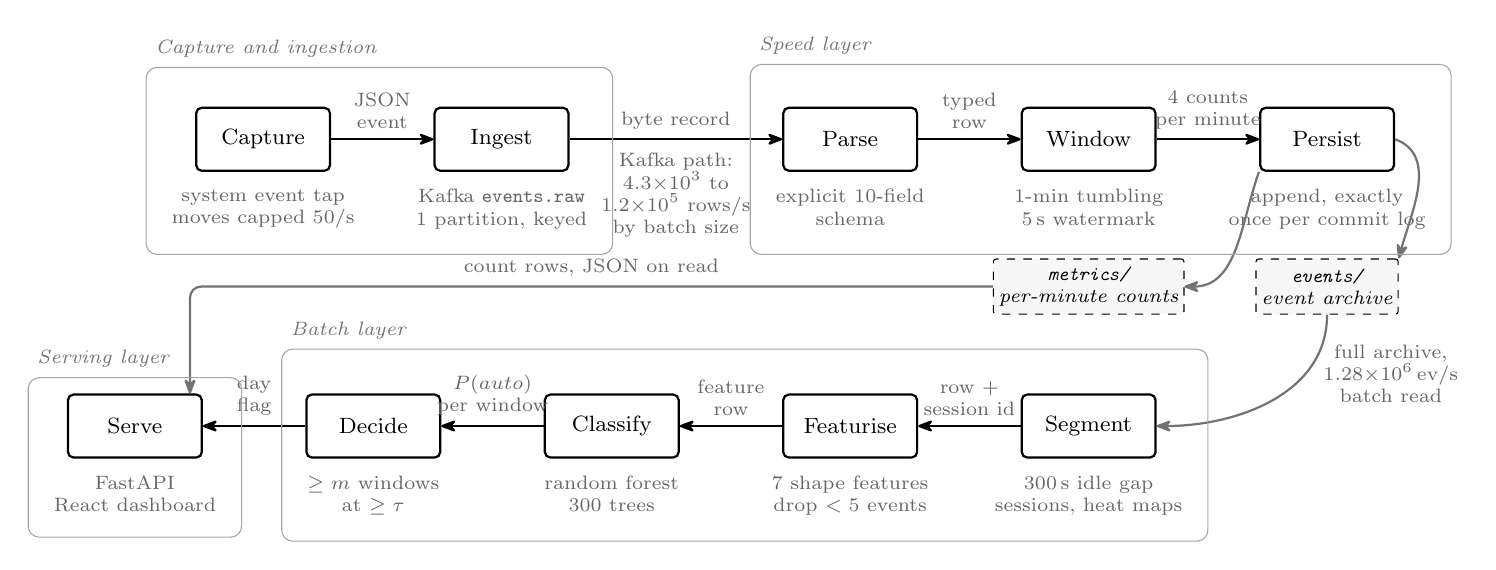
\begin{tikzpicture}[
  >={Stealth[round]},
  font=\footnotesize,
  stage/.style={draw, rounded corners=2pt, align=center, thick,
                minimum height=8mm, minimum width=17mm, inner sep=3pt},
  store/.style={draw, dashed, align=center, font=\scriptsize\itshape,
                rounded corners=1pt, minimum height=7mm, inner sep=2pt,
                fill=black!3},
  note/.style={font=\scriptsize, align=center, text=black!60},
  band/.style={draw=black!35, rounded corners=4pt, inner sep=2mm},
  bandlabel/.style={font=\scriptsize\itshape, text=black!55,
                    anchor=south west},
  flow/.style={->, thick},
  side/.style={->, thick, black!55},
]

% ---- row 1: capture through persistence --------------------------------
\node[stage] (capture)  {Capture};
\node[stage, right=13mm of capture] (ingest)  {Ingest};
\node[stage, right=27mm of ingest]  (parse)   {Parse};
\node[stage, right=13mm of parse]   (window)  {Window};
\node[stage, right=13mm of window]  (persist) {Persist};

\draw[flow] (capture) -- node[above, note] (jsonlab) {JSON\\event} (ingest);
\draw[flow] (ingest)  -- node[above, note] {byte record}
                         node[below, note, yshift=-0.5mm]
                         {Kafka path:\\$4.3{\times}10^{3}$ to\\$1.2{\times}10^{5}$ rows/s\\by batch size} (parse);
\draw[flow] (parse)   -- node[above, note] (typedlab) {typed\\row} (window);
\draw[flow] (window)  -- node[above, note] (cntlab) {4 counts\\per minute} (persist);

\node[note, below=1mm of capture]  (capnote) {system event tap\\moves capped 50/s};
\node[note, below=1mm of ingest]   (ingnote) {Kafka \texttt{events.raw}\\1 partition, keyed};
\node[note, below=1mm of parse]    (parsenote) {explicit 10-field\\schema};
\node[note, below=1mm of window]   (winnote) {1-min tumbling\\5\,s watermark};
\node[note, below=1mm of persist]  (pernote) {append, exactly\\once per commit log};

% ---- the two durable stores --------------------------------------------
\node[store, below=11mm of window]  (metrics) {\texttt{metrics/}\\per-minute counts};
\node[store, below=11mm of persist] (events)  {\texttt{events/}\\event archive};
\draw[side] (persist.south west) to[out=-110, in=0] (metrics.east);
\draw[side] (persist.east) to[out=-20, in=75] (events.north east);

% ---- row 2: the two consumers of the archive ---------------------------
\node[stage, below=10mm of metrics] (segment)   {Segment};
\node[stage, left=13mm of segment]  (featurize) {Featurise};
\node[stage, left=13mm of featurize](classify)  {Classify};
\node[stage, left=13mm of classify] (decide)    {Decide};

\node[note, below=1mm of segment]   (segnote) {300\,s idle gap\\sessions, heat maps};
\node[note, below=1mm of featurize] (featnote) {7 shape features\\drop $<5$ events};
\node[note, below=1mm of classify]  (clsnote) {random forest\\300 trees};
\node[note, below=1mm of decide]    (decnote) {$\geq m$ windows\\at $\geq \tau$};

\draw[side] (events.south) to[out=-90, in=0]
            node[note, right, pos=0.3, xshift=1mm]
            {full archive,\\$1.28{\times}10^{6}$\,ev/s\\batch read}
            (segment.east);
\draw[flow] (segment)   -- node[above, note] (rowlab) {row +\\session id} (featurize);
\draw[flow] (featurize) -- node[above, note] (featlab) {feature\\row} (classify);
\draw[flow] (classify)  -- node[above, note] (pautolab) {$P(\text{auto})$\\per window} (decide);

% ---- serving ------------------------------------------------------------
\node[stage, left=13mm of decide] (serve) {Serve};
\node[note, below=1mm of serve] (servenote) {FastAPI\\React dashboard};
\draw[flow] (decide) -- node[above, note] {day\\flag} (serve);
\draw[side, rounded corners=4pt] (metrics.west) -| ([xshift=7mm]serve.north)
            node[note, above, pos=0.25] {count rows, JSON on read};

% ---- the layer bands ----------------------------------------------------
\node[band, fit=(capture)(ingest)(capnote)(ingnote)(jsonlab)] (captureband) {};
\node[bandlabel] at (captureband.north west) {Capture and ingestion};
\node[band, fit=(parse)(window)(persist)(parsenote)(winnote)(pernote)
             (typedlab)(cntlab)]
     (speedband) {};
\node[bandlabel] at (speedband.north west) {Speed layer};
\node[band, fit=(decide)(classify)(featurize)(segment)
             (decnote)(clsnote)(featnote)(segnote)(pautolab)(featlab)(rowlab)]
     (batchband) {};
\node[bandlabel] at (batchband.north west) {Batch layer};
\node[band, fit=(serve)(servenote)] (serveband) {};
\node[bandlabel] at (serveband.north west) {Serving layer};

\end{tikzpicture}}\end{adjustwidth}
\caption{The KeySpark data flow, following one input event from the operating
system to the dashboard. Grey rounded outlines group the stages into capture
and ingestion, the speed layer, the batch layer, and the serving layer. Solid
arrows carry the record and are labelled with its shape at that point, together
with the measured rate where one exists (Section~\ref{sec:throughput}); the
streaming rate was measured on the deployed path, from a Kafka topic into the
Parquet sinks, over micro-batches of 1,074 to 68,741 rows. Dashed boxes are the two durable stores
through which the speed layer hands records to the batch and serving layers.
The upper row turns an unbounded event stream into finalised per-minute counts;
the lower row consumes the durable archive, where a bounded and fully ordered
view makes order-dependent analytics and automation scoring correct.}
\label{fig:dataflow}
\end{figure}


\subsubsection{Event Capture}
The agent runs as a native host process because the input event tap of the operating system is not reachable from inside a container. It emits one JSON event per input action to the commit log. On wake from sleep the agent exits, so that its restart loop starts a fresh process with a new event tap. An internal watchdog does the same when the operating system reports user activity but the agent has emitted no event for a set time. The capture library also marks events that carry a source process identifier, that is, events injected by software rather than produced by a physical device. The measured deployment discards this mark, so the archive does not distinguish injected from physical input.

\subsubsection{Durable, Replayable Ingestion}
The agent appends each event to a Kafka topic keyed by user~\cite{kreps2011kafka}. This append-only, partitioned log decouples the producer from the consumer in time and rate. It persists events so that a consumer can be restarted or replayed, and it presents the unbounded stream that the streaming engine treats as a growing input table. A single broker runs in Kafka Raft (KRaft) mode inside a container. The producer retries transient failures a limited number of times and is not idempotent, so input events can be lost when the broker is unreachable for long and, in principle, duplicated by a retry.

\subsubsection{Low-Latency Windowed Aggregation}
The speed layer consumes the topic and parses each value with an explicit schema, which avoids the cost and unpredictability of schema inference. Two queries run on this single parsed stream: the first groups events into one-minute tumbling windows per user and aggregates four counts (keystrokes, words, corrections, and clicks), writing each finalised window once. The second writes the parsed events unchanged to the archive used by the batch layer and the classifier.

Four streaming concepts govern correctness. First, windows are defined on the event timestamp rather than on processing time, so a window covers one minute of real activity regardless of ingestion delay. Second, a watermark of five seconds bounds how long the engine waits past the largest observed event time before treating a window as final. Third, the Parquet sink supports only the append output mode, which emits each window's row once and never rewrites it, and which is sound for a windowed aggregation only under a watermark. Let $W$ denote a window, $w$ the watermark duration, and $T_{\max}$ the largest event time observed so far. A window is emitted when
\begin{equation}
T_{\max} - w \;\geq\; \text{end}(W).
\label{eq:emit}
\end{equation}
Because $T_{\max}$ advances only when new events arrive, the last window before a pause is emitted only when activity resumes. Fourth, each query checkpoints its Kafka offsets, and the first also checkpoints its window state. Together with the atomic, log-based commits of the file sink, this gives exactly-once delivery from the Kafka log to the Parquet outputs as recorded in the sink's commit log. A restarted query resumes from its last committed offsets~\cite{armbrust2018structured}. Readers that list part files directly, as the batch job does, bypass that log and can also see files left by an interrupted micro-batch. The guarantee does not extend to the capture side. Besides the producer behaviour above, the source is configured to skip offsets that the broker no longer holds rather than to stop, so events older than the broker's retention are lost after a long outage. Each query runs on a processing-time trigger, of 30\,s for metrics and 60\,s for the archive, which bounds the rate at which files are created.

\subsubsection{Order-Dependent Analytics}
Session boundaries and inter-keystroke timing depend on the previous event. A lag window function computes them in a batch query but does not see across streaming micro-batches, so the same query on the stream would silently miss every gap that straddles a batch boundary. Structured Streaming also offers session windows and arbitrary stateful operators that could carry the previous event per user across micro-batches; these were not used. The design instead computes order-dependent analytics in a batch layer, for three reasons. A batch pass over the archive is simple and takes about two seconds at this data rate; it includes events that arrive behind the watermark (Section~\ref{sec:throughput}); and it can be recomputed when features or models change. The speed layer stores every event durably and emits the simple counts, while a batch job over the bounded archive is the source of truth for order-dependent and session-level analytics. Let the events of a user be ordered by event time as $t_1 \le t_2 \le \dots \le t_n$, and let $G$ be the idle-gap threshold of 300\,s. The session index of the $i$-th event is the running count of session boundaries,
\begin{equation}
s_i \;=\; \sum_{j=1}^{i} \mathbf{1}\!\left[\, j = 1 \;\vee\; t_j - t_{j-1} > G \,\right],
\label{eq:session}
\end{equation}
where $\mathbf{1}[\cdot]$ equals one when its condition holds and zero otherwise; Equation~\eqref{eq:session} is the gaps-and-islands pattern. The batch job also computes per-user baselines, spatial heat maps that bin pointer coordinates into a fixed grid, and per-day metrics for the calendar view of the dashboard. It runs every five minutes and reads the full archive through a file glob, independently of the streaming sink's commit log, so its cost grows with the archive unless reads are made incremental.

\subsubsection{Serving and Operational Resilience}
A small API service reads the Parquet outputs and serves them as JSON to a web dashboard. The dashboard shows live metric cards, per-minute series, heat maps, the session table, and a history calendar that highlights days flagged for automation. Every served field is a count, a timing statistic, or a coordinate bin, so no key identity crosses the API boundary, although the archive behind it still holds key identities. The processing engine runs in local mode because a single user's stream does not require a cluster, and each long-running process is wrapped in a restart loop. A watchdog covers the case in which a host sleep leaves the engine alive but unresponsive. It restarts the streaming and API processes after a wake and otherwise polls the freshness of the batch status and of the streaming output, restarting only the stale component.


\subsection{Automation Detection}
\label{sec:method}

Each one-minute window of the same content-free stream is classified as produced by a person or by input automation. The premise is behavioural: human input is irregular, whereas a jiggler, auto-typer, auto-clicker, or keep-awake tool is regular and repetitive.

\subsubsection{Shape Features}
Seven cross-modal features are computed for each window; they capture regularity rather than volume. Four are dispersion measures. For an ascending sequence of $q$ timestamps with gaps $g_1, \dots, g_{q-1}$, the coefficient of variation (CV) is
\begin{equation}
\mathrm{CV} \;=\; \frac{\sigma_g}{\mu_g},
\label{eq:cv}
\end{equation}
computed with the population standard deviation and defined as zero when fewer than two gaps exist or the mean gap is zero. This convention conflates perfect regularity with the absence of a modality, and the same convention sets \texttt{key\_diversity} and both step features to zero in empty windows. Applying Equation~\eqref{eq:cv} to key-press times, pointer-move times, and the times of all events yields \texttt{ks\_iei\_cv}, \texttt{move\_iei\_cv}, and \texttt{iei\_cv}. Let $K$ be the multiset of key identifiers pressed in the window. Then \texttt{key\_diversity} is the number of distinct identifiers in $K$ divided by $|K|$, which is low for an auto-typer cycling through a small key set and exactly $1/|K|$ for a tool pressing a single key. Pointer geometry is summarised by the Euclidean displacement $d_i$ between consecutive move events: \texttt{step\_mean} is the mean of $d$, and $\texttt{step\_cv} = \sigma_d/\mu_d$ measures how much the step size varies. It is zero for a constant step, for a single step between two moves, and, by the convention above, for a window with fewer than two moves. Finally, for a window with $N$ events of which $N_p$ are pointer events (moves, clicks, and scrolls), $\texttt{mouse\_fraction} = N_p/N$. Windows with fewer than five events carry no shape evidence, because every dispersion measure degenerates to zero and would mimic a perfectly regular tool. Such windows are dropped, so the model abstains on near-empty minutes.

Both \texttt{iei\_cv} and \texttt{mouse\_fraction} pool all event types, and the genuine class contains \texttt{key\_up} and \texttt{scroll} events that the generator below never emits. Hence, the separation could come from event-type composition rather than from human irregularity. Section~\ref{sec:features-models} tests this by recomputing all features from the event types both classes emit.

\subsubsection{Training Classes}
\label{sec:training}
The human class is the genuine archive of Table~\ref{tab:dataset}. The automation class is synthetic, because no captured automation was available. It comprises 16 generated sessions, four of each of four automation kinds (Appendix~\ref{app:generator}, Table~\ref{tab:generator}). The kinds are a mouse jiggler that traces a fixed relative pattern, a slow keep-awake tool that presses a single non-character function key, an auto-typer over a small key set, and an auto-clicker. The jiggler and keep-awake kinds reproduce the input modality and repetition of common keep-active tools, which randomise at most their timing; the auto-typer and auto-clicker are not modelled on a documented tool. The jiggler and keep-awake kinds run faster than the documented defaults, however, so that a one-minute window holds at least five events (Table~\ref{tab:tools}). Each session holds as many events as its base interval gives in 30 minutes, and the inserted pauses stretch it to 50 to 62 minutes. Cadence is jittered per session, and a small amount of cross-modal contamination is added, so that the classes cannot be separated by timing or input mix alone. Generated events enter the evaluation as event records and bypass capture, the move throttle, Kafka, and the speed layer; from the feature extractor on, both classes are processed identically. Section~\ref{sec:slowtools} evaluates the detector on generated sessions that follow the documented defaults instead.

% generated by Paperino/scripts/tooltable.py -- do not edit by hand
\begin{table}[H]
\caption{Default behaviour of real keep-active tools, read from their documentation or source code, against the generator kind that stands for them in training.}
\label{tab:tools}
\centering
\footnotesize
\setlength{\tabcolsep}{3pt}
\begin{adjustwidth}{-\extralength}{0cm}\resizebox{\linewidth}{!}{\begin{tabular}{llrllll}
\toprule
Tool & Platform & Period & Events & Movement & Timing & Generator kind (period, events) \\
\midrule
Mouse Jiggler~\cite{mousejiggler} & Windows & 60\,s & pointer \texttt{move} & relative $(+4,+4)$, then $(-4,-4)$ & optional random timer & \texttt{jiggler}: 1--8\,s \\
Caffeine~\cite{caffeine} & Windows & 59\,s & F15 \texttt{key\_up} & none & none & \texttt{keep\_awake}: 6--12\,s, \texttt{key\_down} \\
Jiggler~\cite{jigglermac} & macOS & 300\,s & burst of 35 \texttt{move} & random, within 14 px & fixed period & not modelled \\
KeepingYouAwake~\cite{keepingyouawake} & macOS & -- & none (power assertion) & none & n/a & invisible by construction \\
\bottomrule
\end{tabular}}\end{adjustwidth}
\par\vspace{2pt}\noindent\footnotesize Period is the documented default; the macOS Jiggler waits for that much idle time before each burst. The generator kinds run about 5 to 60 times faster than these defaults so that a one-minute window holds at least five events. KeepingYouAwake holds a power assertion and emits no input. Movement is the default pattern in the tool's source code. The generator's auto-typer and auto-clicker kinds are not modelled on a documented tool.
\end{table}


\subsubsection{Classification and Decision Policy}
A random forest~\cite{breiman2001random, pedregosa2011scikit} with 300 trees, a minimum of two samples per leaf, balanced class weights, and a fixed random seed (42) scores each window. The simpler learners compared in Section~\ref{sec:features-models} are a logistic regression on standardised features and a decision tree of depth 3, both with balanced class weights. Because a single unusual minute should not determine the label of a whole day, the per-window scores are aggregated into a per-user, per-day decision. The released configuration flags a day $D$ when at least $m = 2$ of its windows score at least $\tau = 0.8$:
\begin{equation}
\bigl|\{\, W \in D \;:\; P(\text{automation} \mid W) \geq \tau \,\}\bigr| \;\geq\; m .
\label{eq:dayflag}
\end{equation}
This rule counts flagged minutes anywhere in the day, so it does not require the sustained burst it is meant to capture. Section~\ref{sec:daypolicy} also evaluates a consecutive rule, which flags a day when at least $r$ flagged windows follow one another within one session. Its window threshold, written $t$ in the tables, is set from the genuine score distribution at a fixed false-positive budget (Section~\ref{sec:protocol}).

\subsection{Evaluation Protocol}
\label{sec:protocol}

The evaluation covers pipeline performance and fault recovery, per-window classification, feature contribution and comparison with other detectors, generalisation across automation kinds, behaviour on real tools' default settings, and the day-level decision policy. Table~\ref{tab:environment} in Appendix~\ref{app:env} lists the hardware and software, and every numeric table and plot is regenerated by a released script.

\textbf{Pipeline.} Batch throughput is measured over three repetitions on the full archive. Streaming throughput is measured as processed rows per second, with three runs per setting, while the number of input files or offsets admitted to each micro-batch is varied. It is measured both by replaying the archived Parquet files into the same windowed aggregation with a no-op sink and on the deployed path from a Kafka topic into the Parquet sinks. Latency from the Kafka topic to the per-minute output is measured with 120 timestamped probe events and compared with the delay that the configuration implies. The processor and memory use of the Spark process and the Kafka container are sampled every second at idle and during a replay. Fault recovery is measured as in Demirezen and Navruz~\cite{demirezen2023lambda}. An archived hour is replayed, by a producer with the agent's settings, through a separate broker while the streaming engine is killed, the broker restarted, offsets lost, and duplicate and late events injected. Per-minute counts are compared with a batch ground truth over three runs per scenario.

\textbf{Classification.} One-minute windows are not independent, because adjacent minutes within one burst share the same rhythm. The synthetic class comprises only 16 sessions, so the effective sample size of the positive class is 16 sessions rather than 645 windows. A hold-out drawn over windows places windows of one session on both sides of the split and partly measures recall of a session already seen. All reported designs therefore hold out whole sessions. The primary design uses four folds that each hold out one synthetic session of every kind and a quarter of the genuine sessions, repeated over ten seeds. Pooled $F_1$ is computed on the out-of-fold predictions of each seed and averaged over the seeds, with a 95\% interval from 1,000 session-level bootstrap replicates. Because each kind has only four sessions, detection is also reported per session, with exact binomial intervals. Ten session-wise random splits that hold out a quarter of all sessions are reported for comparison; they do not control which kinds reach the test set. The positive class is input automation, and $F_1$ is the primary metric, together with precision, recall, and the area under the receiver operating characteristic (ROC) curve (AUC). Leave-one-kind-out (LOKO) folds hold out every session of one kind and use the genuine test partition of the first session-wise split; for the comparison with seen-kind thresholds and for the learning curve, they are repeated over the 40 genuine partitions of the kind-stratified design.

\textbf{Operating points.} A budget threshold is the $(1-b)$ quantile of out-of-fold scores (five-fold, grouped by session) of the genuine training windows, so it uses no automation window. Budgets $b$ of 0.5\%, 1\%, 2\%, and 5\% are evaluated, and day-level counts are reported with Wilson 95\% intervals. The budget and run length were examined on the same days that the grid reports. The forward check therefore refits the detector and threshold on the first 14 genuine days and applies them to the 8 later days. It tests the fitted threshold on unseen days, not the choice of policy, which was made with all days in view.

\textbf{Checks.} The features are recomputed from \texttt{key\_down}, \texttt{move}, and \texttt{click} events only, and separately with a generator that also emits key releases. Generated sessions that follow the documented default settings of real tools are scored by the released detector, with five-minute windows, and with a function-key rule. The windowed keystroke and mouse-dynamics feature set of Wang et al.~\cite{wang2022siurua}, a one-class isolation forest trained on genuine data only, and single-rule baselines are evaluated on the same windows and splits.

\subsection{Use of Generative AI}
Generative AI (Claude Opus 4.8 and Claude Opus 5.5; Anthropic, San Francisco, CA, USA) was used, under the author's direction, to debug analysis scripts, to check the consistency of the event data and of the reported numbers with the script outputs, and to revise and format the manuscript. The author collected the data, reviewed every script and its output, and verified all reported results and references.

%=================================================================
\section{Results}
\label{sec:results}

This section presents the pipeline measurements first and then the detection results, from per-window classification to the day-level decision.

\subsection{Throughput, Latency, and Fault Recovery}
\label{sec:throughput}
As Table~\ref{tab:performance} shows, the batch layer processes the archive in a single in-memory pass at $1.28 \times 10^{6} \pm 0.17 \times 10^{6}$ events per second, much faster per event than the streaming layer because it carries no per-micro-batch overhead.

% generated by Paperino/scripts/sensors_performance.py -- do not edit by hand
\begin{table}[H]
\caption{Processing performance and latency from the Kafka topic to the per-minute output.}
\label{tab:performance}
\centering
\small
\begin{tabular}{lrr}
\toprule
Measure & Value & Variation \\
\midrule
Batch analytics (full archive) & $1.28 \times 10^{6}$ ev/s & $\pm$ $0.17 \times 10^{6}$ \\
Streaming, Parquet replay (4 files) & 29,218 rows/s & 29,185--29,268 \\
Streaming, Kafka path (4,296 rows) & 19,983 rows/s & 19,954--20,028 \\
\midrule Window close to emission (configuration) & 35--65 s & watermark + 1--2 triggers \\
Window close to emission (measured) & 61 s & 60--61 \\
\textbf{Probe event to output (measured)} & \textbf{91 s} & 61--120 \\
\bottomrule
\end{tabular}
\\[2pt] \footnotesize Batch: mean $\pm$ standard deviation of 3 repetitions over the complete 2,962,308-event archive. Streaming: processed rows per second (input rows divided by Spark's \texttt{triggerExecution} time), mean and range of 3 runs at four files, or the same number of rows, per micro-batch (Table~\ref{tab:kafkasweep}). Latency: median and range over 120 probe events (Table~\ref{tab:latency}). The configuration uses one-minute windows, a 5~s watermark, and a 30~s metrics trigger. Probe events are written to the Kafka topic with the agent's producer settings and timed to their window's first appearance in the metrics Parquet output. Window plus watermark alone (65~s) applies only to an event at the start of a minute and leaves out the trigger.
\end{table}


Streaming throughput cannot be summarised by a single number. Figure~\ref{fig:kafkasweep} varies the amount of input admitted to each micro-batch over a 64-fold range, with three runs per setting (Table~\ref{tab:kafkasweep} in Appendix~\ref{app:sweep}). On the Parquet replay, throughput rises from $5.9 \times 10^{3}$ to $2.8 \times 10^{5}$ rows per second, while the mean per-batch latency stays between 145 and 181\,ms up to 32 files per batch. On the deployed path, the job reads the same events from a Kafka topic, parses them, and commits both queries to Parquet sinks with checkpoints. Its throughput is lower at every setting and rises from $4.3 \times 10^{3}$ to $1.2 \times 10^{5}$ rows per second, and its mean per-batch latency grows from 274\,ms at 16-file batches (17,185 rows) to 565\,ms at 64-file batches. Every run lies within 2.2\% of the mean for its setting. This pattern indicates a fixed per-batch cost of query planning, state, and commits, which dominates at small batch sizes and is amortised by larger ones. On the deployed path, per-row work begins to limit the rate above 16-file batches. The observed rate is thus set by micro-batch size rather than by engine speed, and any throughput figure for a micro-batch engine is meaningful only together with the batch size that produced it.

% generated by Paperino/scripts/kafkabench.py -- do not edit by hand
\begin{figure}[H]
\centering
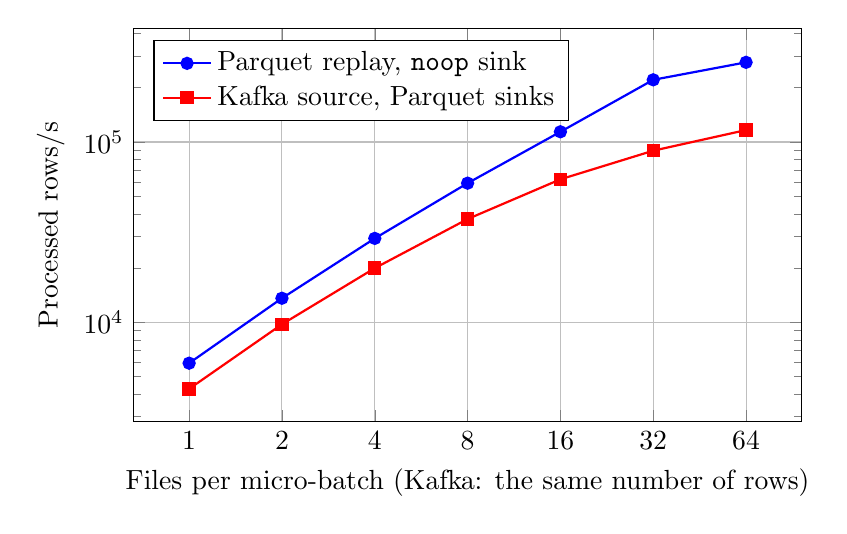
\begin{tikzpicture}
\begin{axis}[
  width=0.70\columnwidth, height=5cm, scale only axis,
  xmode=log, ymode=log, log basis x=2,
  xtick={1,2,4,8,16,32,64}, xticklabels={1,2,4,8,16,32,64},
  xlabel={Files per micro-batch (Kafka: the same number of rows)}, ylabel={Processed rows/s},
  grid=major, legend pos=north west, legend cell align=left,
]
\addplot[mark=*, thick, color=blue, error bars/.cd, y dir=both, y explicit] coordinates {(1,5936) += (0,81) -= (0,90) (2,13605) += (0,251) -= (0,188) (4,29218) += (0,50) -= (0,33) (8,59143) += (0,24) -= (0,17) (16,114009) += (0,1198) -= (0,1511) (32,221381) += (0,1500) -= (0,988) (64,276793) += (0,4661) -= (0,5941)};
\addlegendentry{Parquet replay, \texttt{noop} sink}
\addplot[mark=square*, thick, color=red, error bars/.cd, y dir=both, y explicit] coordinates {(1,4276) += (0,23) -= (0,13) (2,9756) += (0,29) -= (0,46) (4,19983) += (0,45) -= (0,29) (8,37409) += (0,135) -= (0,194) (16,62132) += (0,130) -= (0,238) (32,89549) += (0,474) -= (0,334) (64,116569) += (0,1058) -= (0,736)};
\addlegendentry{Kafka source, Parquet sinks}
\end{axis}
\end{tikzpicture}
\caption{Streaming throughput against micro-batch size from Parquet files and from Kafka (Table~\ref{tab:kafkasweep}); markers give the mean and bars the range of three runs.}
\label{fig:kafkasweep}
\end{figure}


Latency behaves differently. By Equation~\eqref{eq:emit}, a per-minute metric is finalised only after its minute has elapsed and an event at least five seconds past its end has been seen. That event is processed at the next 30\,s trigger, which advances the watermark, and the window is emitted at the trigger after that, so the configuration places emission 35 to 65\,s after the window closes (Table~\ref{tab:performance}). Window and watermark alone, 65\,s for an event at the start of a minute, leave out the trigger and understate the delay. The measurements confirm the full model (Table~\ref{tab:latency} in Appendix~\ref{app:sweep}). Probe events were written to the Kafka topic with the agent's producer settings, so capture is not included, and were timed to their window's first appearance in the metrics Parquet output. For 120 probes sent while a replay kept the stream active, latency ranged from 61 to 120\,s with a median of 91\,s, and 8\% of probes appeared within 65\,s. Every window appeared 60 to 61\,s after it closed, the upper end of the model, because the triggers fell on the full and half minute. When activity paused for five minutes after a probe, its window was not emitted during the pause and appeared 37\,s after the next event, as Equation~\eqref{eq:emit} implies. Per-minute metrics thus trail the activity they describe by one to two minutes, which is acceptable for the per-day decision of Section~\ref{sec:daypolicy} but would matter for an interactive alert. The dashboard adds its own polling delay, which was not measured.

Table~\ref{tab:faults} reports recovery from injected faults. Each scenario replays one archived hour of 55,127 events, the only hour in which all 60 minutes are active, in real time into a private broker, three times, with the deployed job under its restart loop. After a kill of the Spark process, a Java virtual machine (JVM), and after a broker restart, every per-minute count matched the batch ground truth, and no event was lost or duplicated. The job recovered within 18 to 32\,s and 10\,s, respectively. Two of the three kills fell inside a micro-batch. There the first restarted process re-ran the batch and then failed with a \texttt{NullPointerException} in the progress reporting of Spark 4.1.1's Kafka source, and the second restart recovered. These kills also left uncommitted part files, which the sink's commit log excludes but which readers that list every part file, such as the batch job and the API, can see. In these runs such files were truncated or held no duplicate rows, but nothing guarantees that. When the consumer stopped for longer than the broker's retention, 4,460 to 4,474 events expired before they were read and were lost, which the job recorded only as warnings, and window recall fell to 0.917. A block of 200 events sent twice was archived twice, because neither the producer nor the sink removes duplicates. A block of events ten minutes late was dropped from the per-minute counts but kept in the archive, from which the batch layer recovers it. An outage between the producer and the broker, and recovery from host sleep, were not tested.

% generated by Paperino/scripts/faults.py -- do not edit by hand
\begin{table}[H]
\caption{Fault injection on the deployed speed layer.}
\label{tab:faults}
\centering
\small
\setlength{\tabcolsep}{3pt}
\begin{tabular}{lccccccc}
\toprule
 & \multicolumn{2}{c}{Windows} & & \multicolumn{2}{c}{Duplicated} & & \\
\cmidrule(lr){2-3}\cmidrule(lr){5-6}
Scenario & Prec. & Rec. & Lost & Log & Files & Starts & Recovery (s) \\
\midrule
No fault & 1.000 & 1.000 & 0 & 0 & 0 & -- & -- \\
\texttt{kill -9} of the Spark JVM & 1.000 & 1.000 & 0 & 0 & 0 & 1--2 & 18--32 \\
Kafka broker restart & 1.000 & 1.000 & 0 & 0 & 0 & 0 & 10 \\
Offsets lost (retention) & 0.965 & 0.917 & 4,460--4,474 & 0 & 0 & 1 & 5--6 \\
Duplicate block re-sent & 0.967 & 0.967 & 0 & 200 & 200 & -- & -- \\
Block behind the watermark & 0.983 & 0.983 & 0 & 0 & 0 & -- & -- \\
\bottomrule
\end{tabular}
\\[2pt] \footnotesize Each row gives the range over 3 runs. One active archive hour (55,127 events) replayed in real time into a private broker; the deployed job (two queries, Parquet sinks, checkpoints, \texttt{failOnDataLoss=false}) runs under the restart loop of the deployment. Precision and recall are over one-minute windows: a speed-layer window is correct when all four counts equal the batch ground truth. Lost and duplicated events are counted by sequence number in the archive sink, as Spark's commit log records it (log) and as the batch layer and API read it, every part file (files). Starts counts job processes the restart loop launched after the fault. Recovery is the time from the fault (for retention, from the consumer restart) to the commit of the first metrics batch planned after it that read new input, in the job process that then stayed up. Host sleep was not tested.
\end{table}


On the same host, the Spark process used on average 2.4\% of one processor core and at most 888\,MiB of resident memory during a real-time replay of the archived hour (15 events per second on average). At idle it used 0.4\%. The Kafka container used 2.6\% and 1.1\% of one core and at most 755\,MiB. The capture agent's own processor and memory use was not measured.

\subsection{Per-Window Classification}
\label{sec:splits}
Table~\ref{tab:splits} compares a hold-out drawn over windows with one drawn over sessions, and Table~\ref{tab:stratified} reports the kind-stratified design. Holding out sessions instead of windows lowers $F_1$ only from 0.991 to $0.982 \pm 0.009$, which suggests that within-session correlation inflates the window-level estimate only slightly on these data. The spread of the session-wise splits, however, mostly reflects which kinds reach the test set. Their test sets contain 2 to 6 of the 16 synthetic sessions; only one contains all four kinds, and one contains only the jiggler. Under the kind-stratified design, the forest achieves a pooled $F_1$ of 0.988 (95\% interval 0.979 to 0.996) and an AUC of 0.9995, with a recall of at least 0.97 on every kind. At the session level, all four sessions of every kind are detected, with an exact 95\% interval of 40\% to 100\% per kind. The window-level intervals of the jiggler and keep-awake kinds, which have zero width, therefore understate the uncertainty. Once every kind is represented in every test fold, the detector is stable.

% generated by Paperino/scripts/make_tables.py -- do not edit by hand
\begin{table}[H]
\caption{Per-window classification under two hold-out designs.}
\label{tab:splits}
\centering
\footnotesize
\setlength{\tabcolsep}{4pt}
\begin{tabular}{lcc}
\toprule
Metric & Random (window-wise) & Grouped (session-wise) \\
\midrule
Accuracy & 0.997 & 0.996 $\pm$ 0.002 \\
Precision & 0.994 & 0.981 $\pm$ 0.014 \\
Recall & 0.988 & 0.984 $\pm$ 0.021 \\
$F_1$ & 0.991 & 0.982 $\pm$ 0.009 \\
ROC-AUC & 0.9997 & 0.9994 $\pm$ 0.0005 \\
\bottomrule
\end{tabular}
\\[2pt] \footnotesize The positive class is input automation. The grouped split keeps every session entirely on one side, so no window is scored against its own session; its figures are the mean $\pm$ one standard deviation over ten session-wise splits. Counts of true positives, false positives, false negatives, and true negatives: random 159/1/2/912; first grouped split 135/0/6/964.
\end{table}


% generated by paper/scripts/reanalysis_from_csv.py -- do not edit by hand
\begin{table}[H]
\caption{Kind-stratified session-wise evaluation of the forest.}
\label{tab:stratified}
\centering
\small
\begin{tabular}{lcc}
\toprule
Metric & Estimate & 95\% interval \\
\midrule
Pooled $F_1$ & 0.988 & 0.979--0.996 \\
Pooled AUC & 0.9995 & 0.9990--0.9999 \\
Recall, \texttt{jiggler} & 1.000 & 1.000--1.000 \\
Recall, \texttt{typer} & 0.991 & 0.981--1.000 \\
Recall, \texttt{keep\_awake} & 1.000 & 1.000--1.000 \\
Recall, \texttt{clicker} & 0.973 & 0.916--1.000 \\
Fold-mean $F_1$ & 0.988 $\pm$ 0.010 & -- \\
\bottomrule
\end{tabular}
\\[2pt] \footnotesize Each of four folds holds out one synthetic session of every kind and a quarter of the 233 genuine sessions; the design is repeated over ten seeds (40 folds) at threshold 0.5. Pooled values use the out-of-fold scores of all windows, averaged over seeds. Intervals are the 2.5th and 97.5th percentiles of 1,000 session-level bootstrap replicates that resample the genuine sessions and the four sessions of each kind. For comparison, the ten session-wise test sets of Table~\ref{tab:splits} contain 2 to 6 of the 16 synthetic sessions (45 to 263 positive windows); one contains all four kinds and one contains only \texttt{jiggler}. Test sets lacking each kind: \texttt{jiggler} 3, \texttt{typer} 7, \texttt{keep\_awake} 2, \texttt{clicker} 4.
\end{table}


\subsection{Feature Contribution and Comparison with Other Detectors}
\label{sec:features-models}
Permutation importance on the held-out side of the first session-wise split concentrates the signal on \texttt{iei\_cv} (0.707) and \texttt{step\_cv} (0.663) (Table~\ref{tab:features} in Appendix~\ref{app:features}). Over the four kind-stratified folds of the first seed the two are nearly tied (0.647 and 0.643 on average), followed by \texttt{mouse\_fraction} (0.078), and no other feature exceeds 0.03. The importance of \texttt{move\_iei\_cv} falls from a mean decrease in impurity (MDI) of 0.199 to a permutation value of 0.002. Its MDI therefore reflects redundancy with the other dispersion features. \texttt{key\_diversity} contributes almost nothing (0.008 and 0.005 by MDI and permutation, respectively), although it is the most intuitive indicator of an auto-typer.

Table~\ref{tab:ablation} in Appendix~\ref{app:features} compares the forest with simpler learners and with feature blocks under the session-wise splits. The blocks are timing (the three interval CVs), geometry (\texttt{step\_mean} and \texttt{step\_cv}), keyboard (\texttt{key\_diversity} and \texttt{ks\_iei\_cv}), and mouse (\texttt{move\_iei\_cv}, both step features, and \texttt{mouse\_fraction}). A majority-class baseline obtains an accuracy of 0.881 purely because of class imbalance, which is why $F_1$ is the primary metric. Logistic regression and a depth-3 tree achieve $F_1$ scores of $0.804 \pm 0.079$ and $0.852 \pm 0.055$, respectively, compared with $0.982 \pm 0.009$ for the forest. The timing, geometry, and mouse blocks rank the classes almost as well as the full set (AUC 0.9940, 0.9807, and 0.9923, against 0.8868 for the keyboard block), but every block loses $F_1$ at the fixed threshold through lower precision (0.396 to 0.849, against 0.981). Thus, the cross-modal combination mainly improves the operating point rather than discriminative power.


Part of this separation comes from one generator property: for the synthetic class, \texttt{step\_cv} is zero at its 5th, 50th, and 95th percentiles, against a human median of 1.591 (Table~\ref{tab:classdist}), and its median is zero for every kind (Table~\ref{tab:kindfeatures}). It is zero in 631 of 645 synthetic windows (97.8\,\%). In 279 of them the generated moves, those of the jiggler and the contamination moves of the other kinds, repeat a fixed step from the displacement table. In 79 the window holds a single step between two moves, and in the other 273 it has no measurable pointer movement. In genuine windows it is zero in 295 of 3,649 (8.1\,\%), 293 of them without pointer movement. A rule that flags a window whenever \texttt{step\_cv} is zero, with no training, obtains an $F_1$ of $0.727 \pm 0.096$ on the same ten splits and $0.804 \pm 0.040$ under the kind-stratified folds (Table~\ref{tab:baselines}). A rule that flags only windows without pointer movement obtains $0.375 \pm 0.212$ and $0.452 \pm 0.039$, and 0.379 on unseen kinds. The fixed step of the generated moves, a structural property of the generator in the same sense as the missing key releases discussed below, therefore carries most of the rule's power. The \texttt{step\_cv} rule is not far below logistic regression on all seven features. Removing the fixed step does not change the conclusions, however (Table~\ref{tab:geometry} in Appendix~\ref{app:typematched}). In this control, every generated pointer move takes a random step, and all event times, keys, and clicks stay unchanged. Then \texttt{step\_cv} is zero in 54.9\,\% of synthetic windows (the 273 without movement, the 79 single-step windows, and 2 whose random steps happen to be equal). The kind-stratified $F_1$ is 0.985 (95\% interval 0.974 to 0.993), and the leave-one-kind-out mean $F_1$ is 0.439 at the fixed threshold and 0.742 at the 1\% budget. The \texttt{step\_cv} rule, by contrast, falls from 0.804 to 0.547 under the kind-stratified folds and from 0.737 to 0.451 on unseen kinds, while the no-movement rule stays at 0.452 and 0.379.

The separation does not depend on event types the generator lacks (Table~\ref{tab:typematched} in Appendix~\ref{app:typematched}). Recomputing all seven features from \texttt{key\_down}, \texttt{move}, and \texttt{click} events only, for both classes, leaves the session-wise $F_1$ at $0.982 \pm 0.011$ and the kind-stratified $F_1$ at $0.991 \pm 0.005$. The genuine median of \texttt{iei\_cv} falls from 3.756 to 3.351, against 1.267 for the synthetic class, and \texttt{step\_cv} replaces \texttt{iei\_cv} as the most important feature. Adding key releases to the generator instead gives a session-wise $F_1$ of $0.979 \pm 0.011$. The feature ranking, unlike the separation, therefore depends on the event types included.

Table~\ref{tab:baselines} evaluates other detectors on the same windows, sessions, and partitions. With every kind in training, the windowed keystroke and mouse-dynamics features of Wang et al.~\cite{wang2022siurua} perform about as well as the seven shape features (forest $F_1$ $0.977 \pm 0.012$ against $0.988 \pm 0.010$ under the kind-stratified folds). On unseen kinds they score much higher: the forest on these features achieves a leave-one-kind-out mean $F_1$ of 0.958, against 0.459 for the seven shape features. Part of this advantage comes from structural differences between generated and human input rather than from behaviour. Key hold times exist in 80\,\% of genuine windows and in no synthetic window, because the generator emits no key releases. Generated pointer events are also seconds apart, so each forms a one-event action with no path or speed, which the speed features separate trivially. The most important Wang features by permutation are indeed the average speed of move and of point-and-click actions and the mean hold time (\texttt{ata\_move}, \texttt{ata\_point\_click}, and \texttt{hold\_mean} in Table~\ref{tab:baselines}). Without the hold-time features the leave-one-kind-out mean falls to 0.647, still above 0.459; the speed features were not ablated, so how much of the remainder they explain is not known. A one-class isolation forest on the seven features, trained on genuine windows only, ranks the classes with an AUC of 0.950 but obtains an $F_1$ of only $0.561 \pm 0.111$ at its default threshold. On the Wang features it ranks generated windows as more normal than genuine ones (AUC 0.15), consistent with their mostly zero-valued action features lying in a dense region of the genuine distribution. These results indicate that a leave-one-kind-out score against a generator depends strongly on which structural differences between generated and human input a feature set can see. It measures the generator as much as the detector, and the weak cross-kind transfer of the seven shape features need not be inherent to the task. Computing the features through the content-free transform of Section~\ref{sec:capture} changes \texttt{key\_diversity} in 1,387 of 4,294 windows, all through case folding, and leaves the results essentially unchanged ($F_1$ $0.983 \pm 0.009$, leave-one-kind-out mean 0.478; Table~\ref{tab:hardened} in Appendix~\ref{app:hardened}).

% generated by Paperino/scripts/baselines_extra.py from baselines.tex -- do not edit by hand
\begin{table}[H]
\caption{Same-data comparison: the released features against a published keystroke and mouse-dynamics feature set, a one-class detector, and rules.}
\label{tab:baselines}
\centering
\small
\setlength{\tabcolsep}{3pt}
\begin{adjustwidth}{-\extralength}{0cm}\resizebox{\linewidth}{!}{\begin{tabular}{llccccc}
\toprule
 & & \multicolumn{2}{c}{Ten splits} & \multicolumn{2}{c}{Kind-stratified} & LOKO \\
\cmidrule(lr){3-4} \cmidrule(lr){5-6}
Features & Detector & $F_1$ & AUC & $F_1$ & AUC & mean $F_1$ \\
\midrule
Paper (7) & Random forest & 0.982 $\pm$ 0.009 & 0.9994 & 0.988 $\pm$ 0.010 & 0.9995 & 0.459 \\
Paper (7) & Logistic regression & 0.804 $\pm$ 0.079 & 0.9954 & 0.866 $\pm$ 0.027 & 0.9951 & 0.555 \\
Wang et al. (47) & Random forest & 0.967 $\pm$ 0.009 & 0.9999 & 0.977 $\pm$ 0.012 & 0.9998 & 0.958 \\
Wang et al. (47) & Logistic regression & 0.982 $\pm$ 0.010 & 0.9991 & 0.987 $\pm$ 0.007 & 0.9989 & 0.838 \\
Paper (7) & Isolation forest & 0.561 $\pm$ 0.111 & 0.9504 & 0.641 $\pm$ 0.037 & 0.9459 & 0.563 \\
Wang et al. (47) & Isolation forest & 0.000 $\pm$ 0.000 & 0.1519 & 0.000 $\pm$ 0.000 & 0.1458 & 0.000 \\
\texttt{step\_cv} $= 0$ & Rule & 0.727 $\pm$ 0.096 & 0.9376 & 0.804 $\pm$ 0.040 & 0.9488 & 0.737 \\
No pointer movement & Rule & 0.375 $\pm$ 0.212 & 0.6618 & 0.452 $\pm$ 0.039 & 0.6715 & 0.379 \\
Function-key rule & Rule & 0.240 $\pm$ 0.118 & 0.5710 & 0.216 $\pm$ 0.070 & 0.5614 & 0.226 \\
\bottomrule
\end{tabular}}\end{adjustwidth}
\par\vspace{2pt}\noindent\footnotesize Same one-minute windows, sessions, and partitions for every row: ten session-wise splits as in Table~\ref{tab:splits}; four folds that each hold out one synthetic session per kind and a quarter of the genuine sessions, repeated over ten seeds; and leave-one-kind-out (LOKO) with the genuine test sessions of the first split. Wang et al.\ features follow their seven mouse groups (43 values) with keystroke hold and down-down latency summarised by mean and standard deviation; pointer actions are segmented at gaps above 500\,ms, a rule their paper does not specify. Hold times exist in 80\,\% of genuine and 0\,\% of synthetic windows, because the generator emits no \texttt{key\_up}; without them the Wang forest scores $F_1$ 0.975 and LOKO mean 0.647. Its permutation importance is led by \texttt{ata\_move} (0.57), \texttt{ata\_point\_click} (0.47), \texttt{hold\_mean} (0.42). The isolation-forest rows are one-class, trained on genuine windows only. Rules learn nothing; their AUC is that of a binary score. The no-movement rule flags windows without measurable pointer movement (\texttt{step\_mean} $= 0$).
\end{table}


\subsection{Generalisation to Unseen Automation Kinds}
\label{sec:crosskind}
Holding out every session of one kind tests generalisation to a tool absent from training (Table~\ref{tab:crosskind}). The mean $F_1$ falls from 0.988 under the kind-stratified design to 0.459, and the auto-typer is not detected at all ($F_1 = 0$). Precision is 1.000 in every fold that detects anything, so the forest under-scores unseen kinds rather than confusing them with the user. The ranking, however, survives: the AUC stays between 0.9686 and 1.0000 in every fold, and every fold reaches a true-positive rate of one by a false-positive rate of 0.062 (Figure~\ref{fig:roc}).

% generated by Paperino/scripts/make_tables.py -- do not edit by hand
\begin{table}[H]
\caption{Generalisation to an automation kind absent from training: each row holds out every session of one generator kind.}
\label{tab:crosskind}
\centering
\small
\setlength{\tabcolsep}{3pt}
\begin{tabular}{lrrcccc}
\toprule
Held-out kind & Windows & Pos. & Prec. & Rec. & $F_1$ & AUC \\
\midrule
\texttt{jiggler} & 1,106 & 142 & 1.000 & 1.000 & 1.000 & 1.0000 \\
\texttt{typer} & 1,177 & 213 & n/a & 0.000 & 0.000 & 0.9940 \\
\texttt{keep\_awake} & 1,043 & 79 & 1.000 & 0.241 & 0.388 & 0.9686 \\
\texttt{clicker} & 1,175 & 211 & 1.000 & 0.289 & 0.449 & 0.9945 \\
\bottomrule
\end{tabular}
\\[2pt] \footnotesize Mean $F_1$ is 0.459. Training excludes all sessions of the held-out kind and all genuine sessions assigned to test; the genuine test partition is the first session-wise split of Table~\ref{tab:splits}, so the folds are protocol-matched to the grouped row there. Precision is undefined (n/a) when no window is flagged.
\end{table}


% generated by Paperino/scripts/roc_marks.py from roc_crosskind.tex -- do not edit by hand
\begin{figure}[H]
\centering
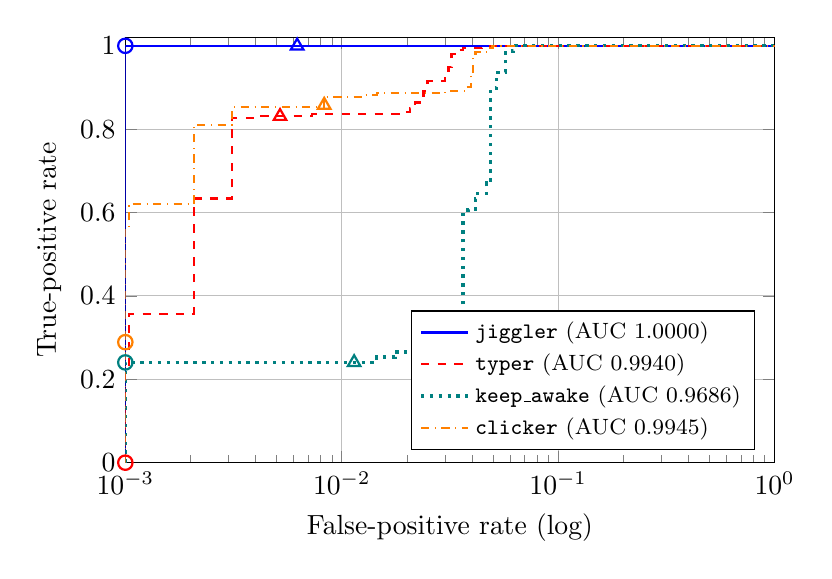
\begin{tikzpicture}
\begin{axis}[
  width=0.68\linewidth, height=5.4cm, scale only axis,
  xmode=log, xmin=0.001, xmax=1, ymin=0, ymax=1.02,
  xlabel={False-positive rate (log)}, ylabel={True-positive rate},
  grid=major, legend pos=south east, legend cell align=left,
  legend style={font=\footnotesize},
]
\addplot[solid, color=blue, thick] coordinates {(0.001,0) (0.001,0.007042) (0.001,0.03521) (0.001,0.07042) (0.001,0.1197) (0.001,0.1338) (0.001,0.2113) (0.001,0.2254) (0.001,0.4577) (0.001,0.5352) (0.001,0.6408) (0.001,0.6831) (0.001,0.7183) (0.001,0.7324) (0.001,0.7676) (0.001,0.7958) (0.001,0.8028) (0.001,0.831) (0.001,0.8451) (0.001,0.8732) (0.001,0.9507) (0.001,0.9859) (0.001,1) (0.01037,1) (0.01245,1) (0.05705,1) (0.05913,1) (0.08817,1) (0.09129,1) (0.09232,1) (0.0944,1) (0.09544,1) (0.1017,1) (0.1037,1) (0.1079,1) (0.1089,1) (0.111,1) (0.1151,1) (0.1172,1) (0.1183,1) (0.1224,1) (0.1234,1) (0.1255,1) (0.1266,1) (0.1369,1) (0.1535,1) (1,1)};
\addlegendentry{\texttt{jiggler} (AUC 1.0000)}
\addplot[dashed, color=red, thick] coordinates {(0.001,0) (0.001,0.004695) (0.001,0.05164) (0.001,0.06103) (0.001,0.07042) (0.001,0.07981) (0.001,0.0939) (0.001,0.1221) (0.001,0.1315) (0.001,0.1408) (0.001,0.169) (0.001,0.1784) (0.001,0.1831) (0.001,0.2066) (0.001,0.216) (0.001037,0.216) (0.001037,0.2582) (0.001037,0.2676) (0.001037,0.2723) (0.001037,0.2864) (0.001037,0.3099) (0.001037,0.3192) (0.001037,0.3568) (0.002075,0.3568) (0.002075,0.3662) (0.002075,0.3803) (0.002075,0.3897) (0.002075,0.3944) (0.002075,0.4085) (0.002075,0.4131) (0.002075,0.4319) (0.002075,0.4507) (0.002075,0.4977) (0.002075,0.5258) (0.002075,0.554) (0.002075,0.5728) (0.002075,0.6103) (0.002075,0.6338) (0.003112,0.6338) (0.003112,0.6526) (0.003112,0.6667) (0.003112,0.6761) (0.003112,0.6854) (0.003112,0.7089) (0.003112,0.7183) (0.003112,0.7418) (0.003112,0.7559) (0.003112,0.7746) (0.003112,0.7887) (0.003112,0.8028) (0.003112,0.8169) (0.003112,0.8263) (0.004149,0.8263) (0.004149,0.831) (0.007261,0.831) (0.007261,0.8357) (0.009336,0.8357) (0.01141,0.8357) (0.01971,0.8357) (0.01971,0.8404) (0.02075,0.8404) (0.02075,0.8498) (0.02178,0.8498) (0.02178,0.8638) (0.02386,0.8638) (0.02386,0.8732) (0.02386,0.892) (0.0249,0.892) (0.0249,0.9014) (0.0249,0.9155) (0.03008,0.9155) (0.03008,0.9202) (0.03008,0.9296) (0.03112,0.9296) (0.03112,0.9343) (0.03112,0.9484) (0.03216,0.9484) (0.03216,0.9765) (0.03216,0.9812) (0.0332,0.9812) (0.0332,0.9906) (0.03631,0.9906) (0.03631,0.9953) (0.04461,0.9953) (0.04461,1) (0.07573,1) (0.0778,1) (0.07988,1) (0.08299,1) (0.0861,1) (0.09025,1) (0.1027,1) (0.1048,1) (0.1255,1) (0.1338,1) (0.1359,1) (0.1369,1) (0.1411,1) (0.1525,1) (1,1)};
\addlegendentry{\texttt{typer} (AUC 0.9940)}
\addplot[dotted, color=teal, very thick] coordinates {(0.001,0) (0.001,0.01266) (0.001,0.02532) (0.001,0.05063) (0.001,0.2405) (0.009336,0.2405) (0.01141,0.2405) (0.01452,0.2405) (0.01452,0.2532) (0.01763,0.2532) (0.01763,0.2658) (0.02178,0.2658) (0.02178,0.2911) (0.02386,0.2911) (0.02386,0.3038) (0.02593,0.3038) (0.02593,0.3418) (0.03631,0.3418) (0.03631,0.5949) (0.03838,0.5949) (0.03838,0.6076) (0.04149,0.6076) (0.04149,0.6329) (0.04253,0.6329) (0.04253,0.6456) (0.04668,0.6456) (0.04668,0.6709) (0.04876,0.6709) (0.04876,0.8987) (0.05187,0.8987) (0.05187,0.9367) (0.05394,0.9367) (0.05602,0.9367) (0.05705,0.9367) (0.05705,0.9494) (0.05705,0.9873) (0.06224,0.9873) (0.06224,1) (0.07054,1) (0.07261,1) (0.08091,1) (0.08299,1) (0.08921,1) (0.09129,1) (0.09959,1) (0.1017,1) (0.1048,1) (0.1089,1) (0.111,1) (0.1203,1) (0.1224,1) (0.1411,1) (0.1452,1) (0.1712,1) (0.1732,1) (0.1743,1) (1,1)};
\addlegendentry{\texttt{keep\_awake} (AUC 0.9686)}
\addplot[dashdotted, color=orange, thick] coordinates {(0.001,0) (0.001,0.004739) (0.001,0.2085) (0.001,0.218) (0.001,0.4076) (0.001,0.4171) (0.001,0.4597) (0.001,0.4692) (0.001,0.5355) (0.001,0.5545) (0.001,0.564) (0.001037,0.564) (0.001037,0.5687) (0.001037,0.5782) (0.001037,0.5972) (0.001037,0.6066) (0.001037,0.6209) (0.002075,0.6209) (0.002075,0.6351) (0.002075,0.6445) (0.002075,0.6588) (0.002075,0.6967) (0.002075,0.7251) (0.002075,0.7393) (0.002075,0.7488) (0.002075,0.7583) (0.002075,0.7678) (0.002075,0.7725) (0.002075,0.8104) (0.003112,0.8104) (0.003112,0.8294) (0.003112,0.8436) (0.003112,0.8531) (0.008299,0.8531) (0.008299,0.8578) (0.008299,0.872) (0.008299,0.8768) (0.01245,0.8768) (0.01245,0.8815) (0.01452,0.8815) (0.01452,0.8863) (0.03008,0.8863) (0.03008,0.891) (0.03734,0.891) (0.03734,0.9005) (0.03942,0.9005) (0.03942,0.9194) (0.03942,0.9289) (0.04046,0.9289) (0.04046,0.9384) (0.04046,0.9526) (0.04046,0.9716) (0.04046,0.9763) (0.04149,0.9763) (0.04149,0.9858) (0.04357,0.9858) (0.04772,0.9858) (0.04772,0.9953) (0.04979,0.9953) (0.04979,1) (0.05187,1) (0.06017,1) (0.06224,1) (0.06639,1) (0.06846,1) (0.07158,1) (0.08091,1) (0.08299,1) (0.08714,1) (0.08921,1) (0.09336,1) (0.09544,1) (0.09647,1) (0.09959,1) (0.1037,1) (0.1214,1) (0.1276,1) (0.1286,1) (0.1369,1) (0.14,1) (1,1)};
\addlegendentry{\texttt{clicker} (AUC 0.9945)}
\addplot[only marks, mark=o, mark size=2.6pt, color=blue, thick, forget plot] coordinates {(0.001,1.0000)};
\addplot[only marks, mark=o, mark size=2.6pt, color=red, thick, forget plot] coordinates {(0.001,0.0000)};
\addplot[only marks, mark=o, mark size=2.6pt, color=teal, thick, forget plot] coordinates {(0.001,0.2405)};
\addplot[only marks, mark=o, mark size=2.6pt, color=orange, thick, forget plot] coordinates {(0.001,0.2891)};
\addplot[only marks, mark=triangle, mark size=2.6pt, color=blue, thick, forget plot] coordinates {(0.006224,1.0000)};
\addplot[only marks, mark=triangle, mark size=2.6pt, color=red, thick, forget plot] coordinates {(0.005187,0.8310)};
\addplot[only marks, mark=triangle, mark size=2.6pt, color=teal, thick, forget plot] coordinates {(0.01141,0.2405)};
\addplot[only marks, mark=triangle, mark size=2.6pt, color=orange, thick, forget plot] coordinates {(0.008299,0.8578)};
\end{axis}
\end{tikzpicture}
\caption{ROC curves of the leave-one-kind-out folds of
Table~\ref{tab:crosskind}, on a logarithmic false-positive axis
(false-positive rates of zero are clipped to $10^{-3}$). Every fold ranks
the classes almost perfectly, including the \texttt{typer} fold whose
$F_1$ at the fixed threshold is zero: the failure is one of operating-point
transfer, not of separability. Circles mark the fixed 0.5 threshold and triangles the 1\%
genuine budget of Table~\ref{tab:transfer}.}
\label{fig:roc}
\end{figure}


The auto-typer differs from the genuine class on several features (Table~\ref{tab:kindfeatures}): its median \texttt{iei\_cv} is 1.336 against 3.756, and its pointer steps are short and constant (\texttt{step\_mean} 4.000 against 18.421, \texttt{step\_cv} zero). Its \texttt{mouse\_fraction} is 0.052 against 0.907, and its AUC stays at 0.994. Its failure at the fixed threshold therefore lies in what the three training kinds teach the forest. None of them combines a mostly keyboard stream with keystroke timing as irregular as a person's: its \texttt{ks\_iei\_cv} median of 1.316 is close to the genuine 1.544 and far from the keep-awake kind's 0.245. The forest trained on them scores every auto-typer window below 0.5.

The failure is thus one of operating-point transfer: the threshold learned against three kinds does not carry over to the fourth. Table~\ref{tab:transfer} tests this directly by setting the threshold from the genuine score distribution alone, without any window of the held-out kind. At a 1\% budget the mean $F_1$ rises from 0.459 to 0.782, with recall of 1.00 on the jiggler, 0.83 on the auto-typer, and 0.86 on the auto-clicker at a per-window false-positive rate of 0.5\% to 1.1\%. At a 5\% budget every kind is recalled in full (mean $F_1$ 0.831), but about 6\% of genuine windows are flagged. The keep-awake kind stays at a recall of 0.24 to 0.25 up to a 2\% budget, because its windows are zero on every pointer feature, a profile that overlaps with sparse keyboard-only human minutes. Of the 3,649 genuine windows, 255 (7.0\%) are keyboard-only, and they make up 19 of the 37 highest-scoring genuine windows (the top 1\%). A one-class isolation forest fitted to genuine data only ranks the held-out kinds with an AUC of 0.904 to 0.969, below the forest. The untrained rule that flags every window with \texttt{step\_cv} $= 0$ reaches a mean $F_1$ of 0.737 on the same held-out kinds (Table~\ref{tab:baselines}). Under the released generator, one artefact without any training thus comes within 0.045 of the budget threshold. With random pointer steps the rule falls to 0.451, whereas the forest keeps 0.742 at the 1\% budget (Table~\ref{tab:geometry}), so most of the forest's score on unseen kinds does not depend on that artefact.

% generated by paper/scripts/reanalysis_from_csv.py -- do not edit by hand
\begin{table}[H]
\caption{Leave-one-kind-out operating points with thresholds set from genuine data only.}
\label{tab:transfer}
\centering
\small
\setlength{\tabcolsep}{3pt}
\begin{tabular}{lccccccc}
\toprule
Threshold & $t$ & \texttt{jiggler} & \texttt{typer} & \texttt{keep\_awake} & \texttt{clicker} & FPR (\%) & Mean $F_1$ \\
\midrule
Fixed 0.5 & 0.50 & 1.00/1.00 & 0.00/0.00 & 0.24/0.39 & 0.29/0.45 & 0.0 & 0.459 \\
0.5\% budget & 0.17--0.31 & 1.00/0.99 & 0.63/0.77 & 0.24/0.37 & 0.85/0.91 & 0.3--0.6 & 0.759 \\
1\% budget & 0.11--0.19 & 1.00/0.98 & 0.83/0.90 & 0.24/0.35 & 0.86/0.91 & 0.5--1.1 & 0.782 \\
2\% budget & 0.08--0.13 & 1.00/0.94 & 0.86/0.88 & 0.25/0.35 & 0.89/0.89 & 1.7--2.3 & 0.766 \\
5\% budget & 0.02--0.03 & 1.00/0.83 & 1.00/0.88 & 1.00/0.72 & 1.00/0.89 & 5.6--6.2 & 0.831 \\
Forest AUC & -- & 1.000 & 0.994 & 0.969 & 0.994 & -- & -- \\
One-class AUC & -- & 0.944 & 0.904 & 0.923 & 0.969 & -- & -- \\
\bottomrule
\end{tabular}
\\[2pt] \footnotesize Leave-one-kind-out folds as in Table~\ref{tab:crosskind}. Kind cells give recall/$F_1$ on the held-out kind against the genuine test partition. A budget threshold is the $(1-b)$ quantile of out-of-fold (five-fold grouped) scores of the genuine training windows, so it uses no window of the held-out kind; $t$ and per-window false-positive rate (FPR) are ranges over the four folds. One-class AUC: an isolation forest (300 trees) fitted to genuine training sessions only, scoring each held-out kind against the same genuine test partition (all kinds pooled: 0.936).
\end{table}


Table~\ref{tab:lokocontrols} adds two controls and repeats the comparison over the 40 genuine partitions of the kind-stratified design. A threshold tuned on the three seen kinds for maximum $F_1$ on out-of-fold training scores gives a mean $F_1$ of 0.483 (0.425 to 0.608 over the partitions). The highest threshold that keeps a recall of at least 0.95 on the seen kinds' out-of-fold scores gives 0.285. Because the seen kinds score high, this threshold reaches up to 0.90, and it detects none of the keep-awake windows. The genuine 1\% budget gives 0.784 (0.765 to 0.803), so tuning on the other kinds does not recover the loss, whereas a threshold set from the genuine distribution does. This is the Neyman--Pearson approach of bounding the false-positive rate on the known class~\cite{tong2018neyman}. Here it is applied to an open-set setting, in which the attack class at test time is not the one seen in training~\cite{scheirer2013openset}. Logistic regression transfers better than the forest at its default threshold (mean $F_1$ 0.588), but at a per-window false-positive rate of 4.6\%. The seen-kind and budget thresholds do not improve it (0.550 to 0.563), and it misses the auto-typer at every operating point.

% generated by Paperino/scripts/review2.py -- do not edit by hand
\begin{table}[H]
\caption{Leave-one-kind-out $F_1$ at thresholds chosen with and without the seen kinds, over 40 genuine partitions.}
\label{tab:lokocontrols}
\centering
\small
\setlength{\tabcolsep}{3pt}
\begin{adjustwidth}{-\extralength}{0cm}\resizebox{\linewidth}{!}{\begin{tabular}{llrrrrrr}
\toprule
Threshold & Model & Jiggler & Typer & Keep-awake & Clicker & Mean $F_1$ (2.5--97.5\%) & FPR \% \\
\midrule
Fixed 0.5 & Forest & 0.99 & 0.00 & 0.38 & 0.48 & 0.464 (0.446--0.496) & 0.1 \\
Fixed 0.5 & Logistic & 0.85 & 0.00 & 0.76 & 0.75 & 0.588 (0.553--0.617) & 4.6 \\
Seen kinds, maximum $F_1$ & Forest & 0.99 & 0.09 & 0.38 & 0.47 & 0.483 (0.425--0.608) & 0.2 \\
Seen kinds, maximum $F_1$ & Logistic & 0.94 & 0.00 & 0.94 & 0.36 & 0.559 (0.522--0.582) & 1.4 \\
Seen kinds, recall $\geq$ 0.95 & Forest & 0.89 & 0.02 & 0.00 & 0.22 & 0.285 (0.204--0.353) & 0.1 \\
Seen kinds, recall $\geq$ 0.95 & Logistic & 0.96 & 0.02 & 0.95 & 0.33 & 0.563 (0.535--0.596) & 1.1 \\
Genuine, 1\% budget & Forest & 0.97 & 0.88 & 0.37 & 0.91 & 0.784 (0.765--0.803) & 0.8 \\
Genuine, 1\% budget & Logistic & 0.97 & 0.00 & 0.95 & 0.28 & 0.550 (0.525--0.575) & 0.9 \\
\bottomrule
\end{tabular}}\end{adjustwidth}
\par\vspace{2pt}\noindent\footnotesize Each held-out kind is tested with the genuine test sessions of every fold of the kind-stratified design (4 folds $\times$ 10 seeds); training uses the other genuine sessions and the three other kinds. Thresholds come from five-fold grouped out-of-fold training scores: the maximum-$F_1$ and recall thresholds use the three seen kinds, the budget uses genuine windows only. Mean $F_1$ is averaged over kinds; the range covers the 40 partitions. FPR is the mean per-window false-positive rate on genuine test windows. Logistic regression is standardised and class-balanced. Mean per-kind AUC over the partitions: forest 0.999 (jiggler), 0.993 (auto-typer), 0.985 (keep-awake), 0.995 (auto-clicker); logistic regression 0.999 (jiggler), 0.952 (auto-typer), 0.994 (keep-awake), 0.966 (auto-clicker).
\end{table}


The size of the synthetic class matters, so Table~\ref{tab:learningcurve} regenerates it with 1 to 32 sessions per kind and five generator seeds and tests every class on the same 40 genuine partitions. The held-out kind's share of the test windows grows with the class, from about 4\% to about 60\%. The table therefore reports the held-out recall and the genuine false-positive rate, which do not depend on that share. It also gives the $F_1$ score at the test composition of the released class. At the 1\% budget the held-out recall stays between 0.72 and 0.83 at every size, at a false-positive rate of 0.85\% to 1.04\%. At the fixed threshold it rises from 0.25 with one session per kind to 0.51 with 32, still well below the budget's. From four sessions on, the seen-kind threshold stays within 0.06 of the fixed one. Only with one session per kind does the seen-kind threshold match the budget (recall 0.76 against 0.72), at about twice the false-positive rate (1.9\% against 1.0\%). Per kind (Table~\ref{tab:learningcurvekinds} in Appendix~\ref{app:learningcurve}), the budget's recall on the jiggler, auto-typer, and auto-clicker barely changes from 2 to 32 sessions, whereas the keep-awake kind's is 0.29 to 0.32 with up to eight sessions and 0.58 and 0.50 with 16 and 32. Generator variability is large: with 16 sessions per kind the budget's mean recall ranges from 0.75 to 0.93 across the five seeds. The headline figures of this paper use the released class of four sessions per kind, which is one draw of this variability.

% generated by Paperino/scripts/learning_curve3.py -- do not edit by hand
\begin{table}[H]
\caption{Leave-one-kind-out detection against the number of generated sessions per kind, over 40 genuine partitions and five generator seeds.}
\label{tab:learningcurve}
\centering
\small
\setlength{\tabcolsep}{3pt}
\begin{adjustwidth}{-\extralength}{0cm}\resizebox{\linewidth}{!}{\begin{tabular}{rrrrrrrrr}
\toprule
Sessions & Synthetic & \multicolumn{3}{c}{Mean held-out recall (2.5--97.5\%)} & FPR (\%) & \multicolumn{3}{c}{Mean $F_1$ at released composition} \\
\cmidrule(lr){3-5} \cmidrule(lr){7-9}
per kind & windows & Fixed 0.5 & Seen kinds & 1\% budget & 1\% budget & Fixed 0.5 & Seen kinds & 1\% budget \\
\midrule
1 & 152--184 & 0.25 (0.16--0.32) & 0.76 (0.54--0.95) & 0.72 (0.53--0.90) & 1.0 & 0.346 & 0.763 & 0.752 \\
2 & 324--353 & 0.37 (0.25--0.44) & 0.56 (0.34--0.76) & 0.75 (0.72--0.85) & 0.9 & 0.459 & 0.627 & 0.795 \\
4 & 645--690 & 0.44 (0.38--0.53) & 0.49 (0.37--0.66) & 0.76 (0.72--0.80) & 0.9 & 0.523 & 0.568 & 0.810 \\
8 & 1,297--1,375 & 0.44 (0.39--0.55) & 0.50 (0.40--0.66) & 0.75 (0.68--0.77) & 0.9 & 0.531 & 0.577 & 0.798 \\
16 & 2,611--2,730 & 0.50 (0.44--0.61) & 0.52 (0.44--0.67) & 0.83 (0.74--0.93) & 0.9 & 0.591 & 0.599 & 0.860 \\
32 & 5,308--5,474 & 0.51 (0.45--0.60) & 0.54 (0.44--0.70) & 0.81 (0.75--0.93) & 0.9 & 0.604 & 0.623 & 0.844 \\
\bottomrule
\end{tabular}}\end{adjustwidth}
\par\vspace{2pt}\noindent\footnotesize Seven-feature random forest. Every size and seed is tested on the 40 genuine test partitions of Table~\ref{tab:lokocontrols}. Thresholds as there: fixed 0.5, the seen-kind maximum-$F_1$ threshold, and the 1\% genuine budget, both from five-fold grouped out-of-fold training scores. Recall is that of the held-out kind and FPR the share of genuine test windows flagged; neither depends on how many windows the held-out kind contributes. $F_1$ at released composition applies the same recall and FPR with the held-out kind weighted to its window count in the released class (142 jiggler, 213 auto-typer, 79 keep-awake, 211 auto-clicker windows). Ranges are the 2.5th and 97.5th percentiles over 200 replicates (40 partitions $\times$ 5 seeds), so they include generator variability. Seed 0 with four sessions per kind is the released class; generated classes of different sizes do not share sessions. Where a grouped inner fold would leave no automation in training, the synthetic sessions are dealt over the inner folds instead (11 of 800 cases at 1 session per kind).
\end{table}


\subsection{Generated Sessions at Real Tools' Default Settings}
\label{sec:slowtools}
As shown in Table~\ref{tab:tools}, the generator runs faster than the tools it stands for. Table~\ref{tab:slowtools} scores generated sessions that follow each tool's documented defaults. The released detector abstains on every minute of Mouse Jiggler at its 60\,s default and of Caffeine at its 59\,s default, because neither reaches five events per minute. It scores 48 of 240 minutes of the macOS Jiggler's idle-triggered bursts but classifies all of them as human. In contrast, five-minute windows recover both Windows tools even when they are absent from training (recall 1.00 when held out), with no day-level false alarms on the 22 genuine days. The cost is a detection delay of at least ten minutes, because the day rule needs two flagged windows and each is scored only after its five minutes close. The per-window false-positive rate also rises about fivefold (9 of 1,017 five-minute windows against 6 of 3,649 one-minute windows), and an unseen macOS Jiggler is still missed (recall 0.29). A rule that flags five consecutive abstained minutes whose key events are all function keys detects Caffeine in every session without false alarms. That holds only because the author's keyboard produced no F1 to F24 key at all (none of 450,473 key events), so the false-alarm figure will not transfer to users who use function keys. All of these sessions are generated: no real tool was run on the capture host, so whether its events reach the agent was not tested.

% generated by Paperino/scripts/slowtools.py -- do not edit by hand
\begin{table}[H]
\caption{Keep-active tools at their default settings: what the released detector scores, and what five-minute windows or an F-key rule recover.}
\label{tab:slowtools}
\centering
\small
\setlength{\tabcolsep}{3pt}
\begin{tabular}{llrcccc c}
\toprule
 & & & \multicolumn{2}{c}{One-minute} & \multicolumn{2}{c}{Five-minute} & F-key \\
\cmidrule(lr){4-5} \cmidrule(lr){6-7}
Tool (default) & Period & Ev./min & Scored & Detected & Scored & Held out / in & rule \\
\midrule
Mouse Jiggler & 60\,s & 1.00 & 0/240 & -- & 44/48 & 1.00 / 1.00 & 0/4 \\
Mouse Jiggler, random timer & 1--60\,s & 1.99 & 1/240 & 1/1 & 48/48 & 1.00 / 1.00 & 0/4 \\
Caffeine (F15 \texttt{key\_up}) & 59\,s & 1.02 & 0/240 & -- & 44/48 & 1.00 / 1.00 & 4/4 \\
Jiggler (macOS), move burst & 300\,s & 2.76 & 48/240 & 0/48 & 48/48 & 0.29 / 1.00 & 0/4 \\
\midrule Genuine windows flagged &  &  &  & 6/3,649 &  & 9/1,017 & -- \\
Genuine days, false alarms &  &  &  & 2/22 &  & 0/22 & 0/22 \\
\bottomrule
\end{tabular}
\\[2pt] \footnotesize Four generated sessions of 60 minutes per tool at its documented defaults. One-minute columns: the released forest (trained on all genuine windows and the 16 synthetic sessions); a window is scored with at least five events; detected means classified as automation by the forest's predicted class (a score strictly above 0.5). Five-minute columns: all classes re-windowed to five minutes; detection is the recall with the tool's sessions held out of training / included as a kind in the kind-stratified folds (one session per kind per fold, 10 seeds). F-key rule: a session or day is flagged after 5 consecutive abstained minutes whose key events are all F1--F24. Genuine row: false alarms of the released day policy ($\tau=0.8$, $m=2$) with genuine windows scored out of fold, and of the rule, out of the genuine days; genuine windows flagged are those classified as automation out of fold (five folds grouped by session). The two Windows tools are modelled on a macOS capture host.
\end{table}


\subsection{Day-Level Decision Policy}
\label{sec:daypolicy}
The dashboard reports a decision per day. For this analysis, genuine windows are scored out of fold in five folds grouped by session, so that no window is scored by a forest trained on its own session. Days are calendar days in Coordinated Universal Time (UTC), assigned by the start of each window. On the capture host (UTC+3), a day thus runs from 03:00 to 03:00 local time, whereas the dashboard's own calendar uses host-local days and the deployed forest. Figure~\ref{fig:calendar} replots the decisions of this section in the dashboard's layout. The four automation days are the three seeded demonstration days (433, 427, and 438 windows) and the test user's day (3 windows). They are scored by the forest trained on all genuine and synthetic windows, which never saw them, giving 22 genuine days and 4 automation days. The seeded days carry the generator's own signature of absent event types, so their detection is not independent evidence that captured automation would be detected. This section is therefore a sensitivity analysis of the decision policy rather than an external validation of the detector.

Table~\ref{tab:daygrid} varies the window threshold and the day rule. The released configuration raises false alarms on 2 of the 22 genuine days (9.1\%, Wilson 95\% interval 2.5\% to 27.8\%), on 8 and 16 June, a rate that the per-window scores do not reveal. Both false alarms consist of isolated flagged minutes, so requiring two consecutive flagged minutes at the same threshold removes them with no change in detection. All six genuine windows that score at least 0.8 lack pointer movement, and two of them are keyboard-only. Their median event count is 73 against 675 for all genuine windows, so the detector confuses sparse, pointer-free minutes with automation. With the window threshold set at a 1\% genuine budget, a run of at least three consecutive flagged minutes gives 1 false alarm in 22 days and 3 detections in 4. By construction, this rule flags a day no earlier than three minutes after automation starts, and scoring on the five-minute batch cycle adds up to five minutes more. This delay was not measured on the deployed path. The count rule at the same threshold flags 10 genuine days. On these 26 days, the fixed 0.8 threshold with two consecutive minutes does as well or better (0 of 22 and 3 of 4). The budget threshold is preferred because it is set from genuine data alone and is the one that transfers to unseen kinds at the window level (Section~\ref{sec:crosskind}). The day counts cannot separate the policies. Detection is 3 of 4 in almost every cell, and the consecutive rules at the fixed thresholds and at budgets up to 1\% differ by at most one false alarm in 22 days. Wherever a day is missed, it is the test user's day, which only the 5\% budget catches, at 4 to 18 false alarms. That day has only three scoreable windows, which leaves almost no margin for any rule that requires a sustained burst. The forward check refits the detector and the 1\% budget threshold (0.211 instead of 0.142) on the first 14 genuine days and their 2,355 windows. On the 8 later days it flags 0.15\% of genuine windows and no genuine day (0 of 8, Wilson 95\% interval 0.0\% to 32.4\%) and detects 3 of the 4 automation days. The released configuration flags 1 of the 8 later days. Scoring the 8 later days as in Table~\ref{tab:daygrid}, with out-of-fold scores and the threshold taken from all 22 days, gives the same counts (0 of 8 under the chosen policy, 1 of 8 under the released configuration, and 3 of 4 detections) and the same per-window rate.

% generated by Paperino/scripts/calendar_plot.py -- do not edit by hand
\begin{figure}[H]
\centering
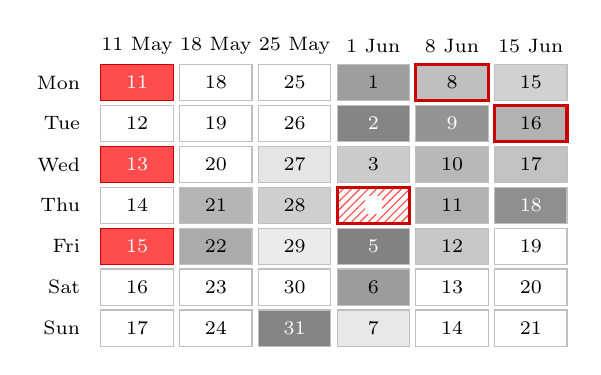
\begin{tikzpicture}[font=\scriptsize]
\node[anchor=east] at (-0.1,0.00) {Mon};
\node[anchor=east] at (-0.1,-0.52) {Tue};
\node[anchor=east] at (-0.1,-1.04) {Wed};
\node[anchor=east] at (-0.1,-1.56) {Thu};
\node[anchor=east] at (-0.1,-2.08) {Fri};
\node[anchor=east] at (-0.1,-2.60) {Sat};
\node[anchor=east] at (-0.1,-3.12) {Sun};
\node at (0.50,0.47) {11 May};
\draw[fill=red!70, draw=red!80!black] (0.04,-0.23) rectangle (0.96,0.23);
\node[text=white] at (0.50,0.00) {11};
\draw[fill=white, draw=black!25] (0.04,-0.75) rectangle (0.96,-0.29);
\node[text=black] at (0.50,-0.52) {12};
\draw[fill=red!70, draw=red!80!black] (0.04,-1.27) rectangle (0.96,-0.81);
\node[text=white] at (0.50,-1.04) {13};
\draw[fill=white, draw=black!25] (0.04,-1.79) rectangle (0.96,-1.33);
\node[text=black] at (0.50,-1.56) {14};
\draw[fill=red!70, draw=red!80!black] (0.04,-2.31) rectangle (0.96,-1.85);
\node[text=white] at (0.50,-2.08) {15};
\draw[fill=white, draw=black!25] (0.04,-2.83) rectangle (0.96,-2.37);
\node[text=black] at (0.50,-2.60) {16};
\draw[fill=white, draw=black!25] (0.04,-3.35) rectangle (0.96,-2.89);
\node[text=black] at (0.50,-3.12) {17};
\node at (1.50,0.47) {18 May};
\draw[fill=white, draw=black!25] (1.04,-0.23) rectangle (1.96,0.23);
\node[text=black] at (1.50,0.00) {18};
\draw[fill=white, draw=black!25] (1.04,-0.75) rectangle (1.96,-0.29);
\node[text=black] at (1.50,-0.52) {19};
\draw[fill=white, draw=black!25] (1.04,-1.27) rectangle (1.96,-0.81);
\node[text=black] at (1.50,-1.04) {20};
\draw[fill=black!29, draw=black!25] (1.04,-1.79) rectangle (1.96,-1.33);
\node[text=black] at (1.50,-1.56) {21};
\draw[fill=black!33, draw=black!25] (1.04,-2.31) rectangle (1.96,-1.85);
\node[text=black] at (1.50,-2.08) {22};
\draw[fill=white, draw=black!25] (1.04,-2.83) rectangle (1.96,-2.37);
\node[text=black] at (1.50,-2.60) {23};
\draw[fill=white, draw=black!25] (1.04,-3.35) rectangle (1.96,-2.89);
\node[text=black] at (1.50,-3.12) {24};
\node at (2.50,0.47) {25 May};
\draw[fill=white, draw=black!25] (2.04,-0.23) rectangle (2.96,0.23);
\node[text=black] at (2.50,0.00) {25};
\draw[fill=white, draw=black!25] (2.04,-0.75) rectangle (2.96,-0.29);
\node[text=black] at (2.50,-0.52) {26};
\draw[fill=black!10, draw=black!25] (2.04,-1.27) rectangle (2.96,-0.81);
\node[text=black] at (2.50,-1.04) {27};
\draw[fill=black!19, draw=black!25] (2.04,-1.79) rectangle (2.96,-1.33);
\node[text=black] at (2.50,-1.56) {28};
\draw[fill=black!8, draw=black!25] (2.04,-2.31) rectangle (2.96,-1.85);
\node[text=black] at (2.50,-2.08) {29};
\draw[fill=white, draw=black!25] (2.04,-2.83) rectangle (2.96,-2.37);
\node[text=black] at (2.50,-2.60) {30};
\draw[fill=black!48, draw=black!25] (2.04,-3.35) rectangle (2.96,-2.89);
\node[text=white] at (2.50,-3.12) {31};
\node at (3.50,0.47) {1 Jun};
\draw[fill=black!38, draw=black!25] (3.04,-0.23) rectangle (3.96,0.23);
\node[text=black] at (3.50,0.00) {1};
\draw[fill=black!48, draw=black!25] (3.04,-0.75) rectangle (3.96,-0.29);
\node[text=white] at (3.50,-0.52) {2};
\draw[fill=black!20, draw=black!25] (3.04,-1.27) rectangle (3.96,-0.81);
\node[text=black] at (3.50,-1.04) {3};
\draw[fill=black!55, draw=red!80!black, line width=1.1pt, pattern=north east lines, pattern color=red!70] (3.04,-1.79) rectangle (3.96,-1.33);
\node[text=white, fill=white, inner sep=1pt] at (3.50,-1.56) {4};
\draw[fill=black!49, draw=black!25] (3.04,-2.31) rectangle (3.96,-1.85);
\node[text=white] at (3.50,-2.08) {5};
\draw[fill=black!39, draw=black!25] (3.04,-2.83) rectangle (3.96,-2.37);
\node[text=black] at (3.50,-2.60) {6};
\draw[fill=black!9, draw=black!25] (3.04,-3.35) rectangle (3.96,-2.89);
\node[text=black] at (3.50,-3.12) {7};
\node at (4.50,0.47) {8 Jun};
\draw[fill=black!25, draw=red!80!black, line width=1.1pt] (4.04,-0.23) rectangle (4.96,0.23);
\node[text=black] at (4.50,0.00) {8};
\draw[fill=black!42, draw=black!25] (4.04,-0.75) rectangle (4.96,-0.29);
\node[text=white] at (4.50,-0.52) {9};
\draw[fill=black!28, draw=black!25] (4.04,-1.27) rectangle (4.96,-0.81);
\node[text=black] at (4.50,-1.04) {10};
\draw[fill=black!30, draw=black!25] (4.04,-1.79) rectangle (4.96,-1.33);
\node[text=black] at (4.50,-1.56) {11};
\draw[fill=black!22, draw=black!25] (4.04,-2.31) rectangle (4.96,-1.85);
\node[text=black] at (4.50,-2.08) {12};
\draw[fill=white, draw=black!25] (4.04,-2.83) rectangle (4.96,-2.37);
\node[text=black] at (4.50,-2.60) {13};
\draw[fill=white, draw=black!25] (4.04,-3.35) rectangle (4.96,-2.89);
\node[text=black] at (4.50,-3.12) {14};
\node at (5.50,0.47) {15 Jun};
\draw[fill=black!18, draw=black!25] (5.04,-0.23) rectangle (5.96,0.23);
\node[text=black] at (5.50,0.00) {15};
\draw[fill=black!30, draw=red!80!black, line width=1.1pt] (5.04,-0.75) rectangle (5.96,-0.29);
\node[text=black] at (5.50,-0.52) {16};
\draw[fill=black!24, draw=black!25] (5.04,-1.27) rectangle (5.96,-0.81);
\node[text=black] at (5.50,-1.04) {17};
\draw[fill=black!44, draw=black!25] (5.04,-1.79) rectangle (5.96,-1.33);
\node[text=white] at (5.50,-1.56) {18};
\draw[fill=white, draw=black!25] (5.04,-2.31) rectangle (5.96,-1.85);
\node[text=black] at (5.50,-2.08) {19};
\draw[fill=white, draw=black!25] (5.04,-2.83) rectangle (5.96,-2.37);
\node[text=black] at (5.50,-2.60) {20};
\draw[fill=white, draw=black!25] (5.04,-3.35) rectangle (5.96,-2.89);
\node[text=black] at (5.50,-3.12) {21};
\end{tikzpicture}
\caption{Day-level decisions of the released configuration ($\tau = 0.8$, $m \geq 2$), replotted from the released feature table in the layout of the dashboard's history calendar. Days are UTC calendar days from 11 May to 21 June 2026; grey shading gives the number of scored genuine windows that day (darkest 347). Genuine windows are scored out of fold. Red fill: automation days detected (11 May, 13 May, 15 May); red hatching: the test user's day, not detected (4 June), which also holds genuine activity; red outline: genuine days flagged (8 June, 16 June).}
\label{fig:calendar}
\end{figure}


% generated by paper/scripts/reanalysis_from_csv.py -- do not edit by hand
\begin{table}[H]
\caption{Day-level false alarms and detections by window threshold and day rule.}
\label{tab:daygrid}
\centering
\small
\setlength{\tabcolsep}{4pt}
\begin{tabular}{lccccccc}
\toprule
 & & \multicolumn{3}{c}{Count, $m \geq$} & \multicolumn{3}{c}{Consecutive, $r \geq$} \\
\cmidrule(lr){3-5}\cmidrule(lr){6-8}
Threshold & $t$ & 2 & 3 & 5 & 2 & 3 & 5 \\
\midrule
Fixed 0.5 & 0.500 & 2/3 & 0/3 & 0/3 & 0/3 & 0/3 & 0/3 \\
Fixed 0.8 & 0.800 & \underline{2/3} & 0/3 & 0/3 & 0/3 & 0/3 & 0/3 \\
0.5\% budget & 0.236 & 6/3 & 2/3 & 0/3 & 0/3 & 0/3 & 0/3 \\
1\% budget & 0.142 & 10/3 & 7/3 & 1/3 & 1/3 & \textbf{1/3} & 0/3 \\
2\% budget & 0.097 & 15/3 & 13/3 & 5/3 & 3/3 & 1/3 & 0/3 \\
5\% budget & 0.044 & 18/4 & 18/4 & 13/3 & 11/4 & 4/4 & 0/3 \\
\bottomrule
\end{tabular}
\\[2pt] \footnotesize Cells give false alarms out of 22 genuine days / detections out of 4 automation days. Window scores as in Section~\ref{sec:daypolicy}: genuine windows out of fold, automation days by the forest fitted to all genuine and synthetic windows. A window is flagged when its score is at least $t$; a budget threshold is the $(1-b)$ quantile of the out-of-fold genuine scores. A day is flagged when at least $m$ of its windows are flagged (count) or when at least $r$ flagged windows follow one another within one session (consecutive). Underlined is the released configuration, bold the operating point checked forward in time in Section~\ref{sec:daypolicy}. Wilson 95\% intervals (\%): 0/22, 0.0--14.9; 1/22, 0.8--21.8; 2/22, 2.5--27.8; 3/22, 4.7--33.3; 4/22, 7.3--38.5; 5/22, 10.1--43.4; 6/22, 13.2--48.2; 7/22, 16.4--52.7; 10/22, 26.9--65.3; 11/22, 30.7--69.3; 13/22, 38.7--76.7; 15/22, 47.3--83.6; 18/22, 61.5--92.7; 3/4, 30.1--95.4; 4/4, 51.0--100.0.
\end{table}



%=================================================================
\section{Discussion}
\label{sec:discussion}

\subsection{Interpretation of the Findings}
For the pipeline, the results show that standard stream-processing components can capture, transport, and analyse a continuous input-event stream end to end. The speed layer's per-minute counts survived a killed engine and a restarted broker without loss or duplication (Table~\ref{tab:faults}). The failures that did occur are the ones its configuration permits: events lost when offsets expire, duplicates passed through from the producer side, and late events left to the batch layer. Streaming throughput is governed by micro-batch size rather than engine speed. On the Parquet replay it rose from $5.9 \times 10^{3}$ to $2.8 \times 10^{5}$ rows per second over a 64-fold change in batch size. The mean per-batch latency meanwhile stayed between 145 and 181\,ms up to 32 files per batch, which identifies a fixed per-batch cost as the limiting factor at small batch sizes. The measured latency of one to two minutes agrees with the full configuration, in which the trigger schedule adds about one minute to window and watermark; window and watermark alone understate it. The Lambda split is a design choice rather than a necessity, because stateful streaming operators could also compute sessions. A batch pass over the archive is simple at this data rate, keeps late events, and can be recomputed. This agrees with the role of the batch layer as the source of truth in other sensor applications of the architecture~\cite{demirezen2023lambda, khattach2025iot}.

For detection, H1 holds on this subject for the generated kinds. The user's input is more irregular than the generated automation, the separation survives when both classes are restricted to the same event types, and it is stable once every kind appears in every test fold. Against the named baselines, the forest's kind-stratified $F_1$ of 0.988 exceeds that of logistic regression on the same features (0.866) and of the best rule (\texttt{step\_cv} $= 0$, 0.804). It matches the feature set of Wang et al.\ (0.977 and 0.987; Table~\ref{tab:baselines}). Part of it rests on the fixed step of the generated pointer moves (\texttt{step\_cv}), although a generator with random steps leaves the separation and the transfer results almost unchanged. H1 is not supported for generated sessions at real tools' default settings, which the one-minute detector abstains on or classifies as human. H2 fails at the fixed threshold, because a detector trained on some automation kinds under-scores the others. It is partly supported at the 1\% budget (mean $F_1$ 0.782 against 0.988 in the kind-stratified design, with the keep-awake kind's $F_1$ still at 0.35 and its recall at 0.24). The distinction between ranking and operating point is the central result for the forest. Unseen kinds stay almost perfectly ranked, and thresholds tuned on the seen kinds do not transfer. A threshold set from the genuine score distribution, which can be estimated without any automation data, raises held-out recall well above the fixed and seen-kind thresholds at every synthetic-class size from 2 to 32 sessions per kind. With one session per kind a seen-kind threshold does as well, at about twice the false-positive rate. Under the released generator, an untrained rule on \texttt{step\_cv} comes within 0.045 of the budget threshold on unseen kinds. With random pointer steps, however, the rule falls to 0.451 while the forest keeps 0.742, so this result does not rest on the fixed-step artefact. Bounding the false-positive rate on the known class is standard in Neyman--Pearson classification~\cite{tong2018neyman}, and the budget threshold delivers that for both models (0.8\% and 0.9\% of genuine windows). Only for the forest does it also recover $F_1$ on unseen kinds. Logistic regression ranks the auto-typer less well (AUC 0.952), and its auto-typer windows do not score above the top 1\% of genuine windows, so the same threshold leaves it below its default (0.550 against 0.588).

The same design also ranks feature sets differently from a conventional hold-out. With every kind in training, the seven shape features and the windowed feature set of Wang et al.~\cite{wang2022siurua} perform alike. On unseen kinds the richer set scores far higher (leave-one-kind-out mean $F_1$ 0.958 against 0.459), partly through the generator's missing key releases: without hold times it falls to 0.647. The rest of the gap is consistent with the generator's discontinuous pointer events, which were not ablated. The recent input-based bot-detection studies of Table~\ref{tab:related} report no hold-out of whole automation kinds, so neither effect is visible there. The results suggest that such detectors should be thresholded from genuine data, which bounds the false-positive rate, compared on held-out automation kinds, and checked for features that separate the generator's structure rather than its behaviour.

\subsection{Limitations}
This study has several limitations, each stated below with the direction in which it biases the results and the analysis that bounds it.

\textbf{Single subject.} The corpus covers one user on one machine, so no cross-user claim is made. The genuine false-alarm rates would likely be higher for users whose input is less bursty or who use function keys. The forward hold-out bounds drift over time for this user: a detector fitted on the first 14 days falsely flagged 0.15\% of later genuine windows and, under the chosen policy, none of the 8 later days.

\textbf{Synthetic automation class.} The automation class is generated, and no real tool was captured, so the scores partly measure separation from a particular generator. Its pointer moves repeat a fixed step, which makes \texttt{step\_cv} exactly zero and inflates separability, and its missing key releases make hold-time features trivially separating. The leave-one-kind-out, threshold-transfer, random-step, and hold-time-free comparisons bound how much of the performance depends on having seen a kind or on these artefacts; human-like generated trajectories were not tested. Each kind has four sessions, so per-kind results carry wide session-level intervals (40\% to 100\% for four of four). The leave-one-kind-out scores depend on the number and the draw of generated sessions: from 1 to 32 sessions per kind the held-out recall at the fixed threshold rises from 0.25 to 0.51 without reaching the budget's 0.72 to 0.83, and with 16 sessions per kind the budget's recall varies from 0.75 to 0.93 across generator seeds (Table~\ref{tab:learningcurve}).

\textbf{Default cadence.} The generator runs about 5 to 60 times faster than the documented defaults of the tools it stands for, so the one-minute results apply to fast-cadence automation. At default settings the detector abstains on the Windows tools and misses the macOS Jiggler (Section~\ref{sec:slowtools}).

\textbf{Window design.} The one-minute window and the five-event minimum were not varied for the main results. They set the coverage boundary for slow tools, and only five-minute windows were tested, for those tools alone; how the kind-stratified and leave-one-kind-out results depend on either setting is not known.

\textbf{Event-type mix and capture throttle.} The generator emits no \texttt{key\_up} and no \texttt{scroll} events, which make up 7.9\,\% and 41.9\,\% of the genuine archive, and the 20\,ms move throttle clamps pointer timing in the genuine class. The type-matched features show that the separation does not depend on the missing event types, although the feature ranking does. \texttt{move\_iei\_cv} partly measures the throttle, but its permutation importance is only 0.002, so this has little effect on the results.

\textbf{Day-level evidence.} The day-level analysis rests on 4 automation days that share the generator's signature, so its detection rate has a wide interval (30\% to 95\%). The operating point was also chosen with these days in view; the forward check tests the refitted threshold on later days but not the choice of policy.

\textbf{Pipeline scope.} All measurements come from one host in local mode, so partitioning and shuffle behaviour across machines is not exercised. The fault tests replay one hour three times per scenario and bound, rather than prove, the recovery behaviour. Recovery from host sleep and the capture agent's own processor and memory use were not measured.

Two further boundaries apply to any detector that operates on the input stream. Keep-awake tools that only hold a power assertion, such as PowerToys Awake~\cite{powertoysawake} and KeepingYouAwake~\cite{keepingyouawake}, emit no input events, so they are invisible by construction. A hardware jiggler that also randomises its timing remains the hard case, detectable, if at all, only by its geometry.

\subsection{Future Work}
Future work will first validate the detector against captured automation, starting with the macOS Jiggler on the capture host. Software keep-active tools post synthetic events into the system's event stream, and the capture library marks events that carry a source process identifier as injected~\cite{pynput}. Whether a given tool's events reach the agent's tap was not tested here. If they do, recording that mark is a content-free way to separate software automation from physical input. The behavioural detector would then cover hardware devices whose events arrive as physical input, and a hardware jiggler is the natural source of captured automation for that case. Public mouse-dynamics corpora with raw $(x, y, t)$ traces would provide an external genuine population for the false-alarm rate. Longer windows, or a key-class feature computed through the content-free transform, would extend coverage to slow tools. A multi-user, clustered deployment would exercise partitioning and shuffle behaviour. All of these directions require moving the content-free capture transform into the agent first, so that typed characters never reach the log.

%=================================================================
\section{Conclusions}
\label{sec:conclusions}

This paper presented KeySpark, a streaming pipeline for keyboard and mouse events with content-free analytics and features, and used it to study whether input automation can be detected continuously from the event stream of one user. A Lambda architecture separates low-latency per-minute metrics from order-dependent, session-level analytics. Streaming throughput was governed by micro-batch size. The per-minute counts survived a killed engine and a restarted broker without loss or duplication. Events were lost when offsets expired, a re-sent block was archived twice, an outage between producer and broker was not tested, and the latency from the Kafka topic to the per-minute output was one to two minutes. A random forest on seven content-free features separated the user's input from four kinds of generated automation with an $F_1$ of 0.988 when every kind appeared in training and testing. The separation held when both classes were restricted to the same event types or when the generated pointer moves took random steps. When a kind was absent from training, the fixed threshold failed (mean $F_1$ 0.459) while the ranking survived (AUC above 0.96). For this forest, a threshold set from genuine data alone raised the mean $F_1$ to 0.782, whereas thresholds tuned on the seen kinds did not. Over 40 partitions and five generator seeds, it kept held-out recall at 0.75 to 0.83 from 2 to 32 generated sessions per kind, against at most 0.56 for the other thresholds. For logistic regression it bounded the false-positive rate without recovering $F_1$. The windowed feature set of Wang et al.\ reached 0.958 on the same folds, partly through structural artefacts of the generator. A consecutive-minute day rule at the genuine-data threshold, refitted on earlier days, flagged none of the later genuine days. For this detector and generator, holding out whole automation kinds changed the conclusions, and a threshold set from genuine data was needed to detect unseen kinds. Generated sessions at real tools' default settings were abstained on or missed, so slow tools need longer windows or capture-level signals. No real tool was captured, and whether tools' events reach the capture tap is untested, so validation against captured automation remains the next step.

%=================================================================
\vspace{6pt}

\authorcontributions{Conceptualization, methodology, software, validation, formal analysis, investigation, data curation, writing (original draft preparation), writing (review and editing), and visualization, M.E.A. The author has read and agreed to the published version of the manuscript.}

\funding{This research received no external funding.}

\institutionalreview{Ethical review and approval were waived for this study because the only participant is the author, who recorded the input events of their own computer during their own work; no data from any other person were collected. The raw event archive is kept only on the author's computer and will be deleted after publication, and only content-free per-window features are released.}

\informedconsent{Not applicable; the only data subject is the author of this study.}

\dataavailability{The source code of the pipeline and a content-free per-window feature table are openly available at \url{https://github.com/Hanceptron/KeySpark}. The table holds the seven features, labels, session identifiers, and day indices of all 3,649 genuine, 645 synthetic, and 1,301 automation-day windows used in this study, without key identities, typed text, pointer coordinates, or clock times. Its 233 genuine sessions are fewer than the 242 of Table~\ref{tab:dataset} because nine sessions contain only windows with fewer than five events, which the detector drops. The table reproduces the session-wise, kind-stratified, leave-one-kind-out, operating-point, and day-level results of Section~\ref{sec:results}. The raw event archive is not available, because it contains the plaintext keystrokes of the author, which may include text about other people, and whether the content-free transform prevents recovery of that text was not assessed. The archive-based results can therefore be rerun only by the author, and not after the archive is deleted: Tables~\ref{tab:dataset}, \ref{tab:performance}, \ref{tab:faults}, \ref{tab:typematched}, \ref{tab:hardened}, \ref{tab:kafkasweep}, and~\ref{tab:latency}; Figure~\ref{fig:day}; the Wang et al.\ and function-key rows of Table~\ref{tab:baselines}; the five-minute and function-key columns of Table~\ref{tab:slowtools}; and the count of function keys among the 450,473 genuine key events.}

\acknowledgments{During the preparation of this manuscript, the author used Claude (Opus 4.8 and Opus 5.5; Anthropic, San Francisco, CA, USA) for the purposes of debugging analysis scripts under the author's direction, checking the consistency of the event data and reported numbers, revising the text, language refinement, and LaTeX formatting. The author has reviewed and edited the output and takes full responsibility for the content of this publication.}

\conflictsofinterest{The author declares no conflicts of interest.}

\abbreviations{Abbreviations}{%
The following abbreviations are used in this manuscript:\\

\noindent
\begin{tabular}{@{}ll}
API & Application programming interface\\
AUC & Area under the ROC curve\\
CV & Coefficient of variation\\
FPR & False-positive rate\\
GAN & Generative adversarial network\\
HID & Human interface device\\
JSON & JavaScript Object Notation\\
JVM & Java virtual machine\\
KRaft & Kafka Raft\\
LOKO & Leave-one-kind-out\\
MDI & Mean decrease in impurity\\
ROC & Receiver operating characteristic\\
UTC & Coordinated Universal Time
\end{tabular}
}

%=================================================================
\appendixtitles{yes}
\appendixstart
\appendix

\section{Generator Settings}
\label{app:generator}
% generated by Paperino/scripts/generator_table.py -- do not edit by hand
\begin{table}[H]
\caption{Settings of the synthetic automation generator.}
\label{tab:generator}
\centering
\small
\setlength{\tabcolsep}{3pt}
\begin{tabular}{lrp{6.6cm}rr}
\toprule
Kind & Interval & Events & Minutes & Windows \\
\midrule
\texttt{jiggler} & 1--8\,s & pointer \texttt{move} walking one fixed pattern per session: diagonal (2 steps, at most 4\,px per axis), horizontal (2 steps, at most 4\,px per axis), octagon (8 steps, at most 3\,px per axis), scaled by 1 to 3 & 51--54 & 142 \\
\texttt{typer} & 0.1--0.4\,s & \texttt{key\_down} over 8 keys (a, s, d, f, j, k, l, e) & 51--53 & 213 \\
\texttt{keep\_awake} & 6--12\,s & \texttt{key\_down} of one key per session (F15, F13, F14, Scroll Lock) & 50--62 & 79 \\
\texttt{clicker} & 0.3--1.5\,s & left \texttt{click} at the current pointer position & 51--54 & 211 \\
\bottomrule
\end{tabular}
\\[2pt] \footnotesize Four sessions per kind. Per session the generator draws the base interval between events from the range shown, a timing jitter of 20\% to 50\% of it, and the pattern, distance, or key. Each session holds as many events as its base interval gives in 30 minutes; 10\% of intervals are lengthened by 3 to 12 base intervals as pauses, which stretches a session to the length shown. 8\% of events are drawn from another kind (cross-modal contamination). No kind emits \texttt{key\_up} or \texttt{scroll}. Windows are the one-minute windows with at least five events.
\end{table}


\section{Evaluation Environment}
\label{app:env}
% generated by Paperino/scripts/make_tables.py -- do not edit by hand
\begin{table}[H]
\caption{Evaluation environment.}
\label{tab:environment}
\centering
\begin{tabular}{ll}
\toprule
Component & Version \\
\midrule
Processor & Apple M5 Max, 18 cores \\
Memory & 128 GB \\
Operating system & macOS 26.5.2 \\
Java runtime & OpenJDK 21.0.11 LTS \\
Apache Spark & 4.1.1 (Scala 2.13.17) \\
Apache Kafka & 3.8.1, KRaft, single broker \\
Python & 3.12.13 \\
scikit-learn & 1.8.0 \\
\bottomrule
\end{tabular}
\\[2pt] \footnotesize Spark runs in \texttt{local[*]} mode; Kafka runs in a container.
\end{table}


\section{Throughput Sweep and Latency}
\label{app:sweep}
% generated by Paperino/scripts/kafkabench.py -- do not edit by hand
\begin{table}[H]
\caption{Streaming throughput against micro-batch size, from Parquet files and from Kafka.}
\label{tab:kafkasweep}
\centering
\small
\setlength{\tabcolsep}{3pt}
\begin{tabular}{rrrrrr}
\toprule
 & & \multicolumn{2}{c}{Processed rows/s} & \multicolumn{2}{c}{Mean batch ms} \\
\cmidrule(lr){3-4}\cmidrule(lr){5-6}
Files & Rows/batch & Parquet & Kafka & Parquet & Kafka \\
\midrule
1 & 1,074 & 5,936 (5,846--6,017) & 4,276 (4,263--4,299) & 181 & 251 \\
2 & 2,148 & 13,605 (13,417--13,856) & 9,756 (9,710--9,784) & 158 & 220 \\
4 & 4,296 & 29,218 (29,185--29,268) & 19,983 (19,954--20,028) & 147 & 215 \\
8 & 8,593 & 59,143 (59,126--59,167) & 37,409 (37,215--37,544) & 145 & 229 \\
16 & 17,185 & 114,009 (112,498--115,207) & 62,132 (61,894--62,262) & 149 & 274 \\
32 & 34,371 & 221,381 (220,393--222,881) & 89,549 (89,215--90,023) & 152 & 376 \\
64 & 68,741 & 276,793 (270,852--281,454) & 116,569 (115,833--117,627) & 238 & 565 \\
\bottomrule
\end{tabular}
\\[2pt] \footnotesize Mean (min--max) over 3 runs per point. Both series replay the 2,962,308 events of the complete archive. Parquet: the streaming replay (files from disk, the windowed aggregation, a \texttt{noop} sink). Kafka: the same events preloaded into a Kafka topic and read by the deployed parse and both queries (windowed counts and archive), each with a Parquet sink and checkpoint, \texttt{maxOffsetsPerTrigger} set to the rows of the given number of files; rows/s is the windowed-count query's processed rate while the archive query runs alongside. Batch latency is the mean \texttt{triggerExecution} time of that query.
\end{table}

% generated by Paperino/scripts/kafkabench.py -- do not edit by hand
\begin{table}[H]
\caption{Measured latency of the speed layer from the Kafka topic to the per-minute output.}
\label{tab:latency}
\centering
\small
\begin{tabular}{lrrrr}
\toprule
Probes & Min & Median & 95th pct. & Max \\
\midrule
All probes ($n=120$) & 61 & 91 & 118 & 120 \\
Sent at second 0--15 ($n=27$) & 106 & 113 & 119 & 120 \\
Sent at second 15--30 ($n=33$) & 91 & 100 & 104 & 105 \\
Sent at second 30--45 ($n=31$) & 76 & 83 & 90 & 90 \\
Sent at second 45--60 ($n=29$) & 61 & 67 & 75 & 76 \\
\bottomrule
\end{tabular}
\\[2pt] \footnotesize Seconds from sending a probe event to its window's first appearance in the metrics Parquet output, with a real-time archive replay keeping the stream active. Every window appeared 60 to 61~s after it closed (median 61~s), so latency falls with the probe's second in the minute; 8\% of probes appeared within 65~s, the window plus the watermark. When activity paused for 5~min after a probe, its window was not emitted during the pause; it appeared 37~s after the next event, 340~s after it was sent.
\end{table}


\section{Features, Learners, Distributions, and Per-Kind Medians}
\label{app:features}
% generated by Paperino/scripts/make_tables.py -- do not edit by hand
\begin{table}[H]
\caption{Per-window shape features, ranked by importance.}
\label{tab:features}
\centering
\footnotesize
\setlength{\tabcolsep}{3pt}
\begin{tabular}{llrr}
\toprule
Feature & Definition & MDI & Perm. \\
\midrule
\texttt{step\_cv} & CV of pointer step size & 0.317 & 0.663 \\
\texttt{iei\_cv} & CV of all inter-event intervals & 0.279 & 0.707 \\
\texttt{move\_iei\_cv} & CV of inter-move intervals & 0.199 & 0.002 \\
\texttt{step\_mean} & mean pointer step, pixels & 0.090 & 0.012 \\
\texttt{ks\_iei\_cv} & CV of inter-keystroke intervals & 0.066 & 0.004 \\
\texttt{mouse\_fraction} & mouse events per event & 0.041 & 0.122 \\
\texttt{key\_diversity} & distinct keys per keystroke & 0.008 & 0.005 \\
\bottomrule
\end{tabular}
\\[2pt] \footnotesize Rows follow MDI. MDI is mean decrease in impurity over the forest fitted to all windows; Perm.\ is $F_1$-scored permutation importance on the held-out side of the first session-wise split (20 shuffles). CV denotes the coefficient of variation.
\end{table}

% generated by Paperino/scripts/make_tables.py -- do not edit by hand
\begin{table}[H]
\caption{Classifier and feature-block comparison, session-wise hold-out.}
\label{tab:ablation}
\centering
\small
\setlength{\tabcolsep}{3pt}
\begin{tabular}{lccccc}
\toprule
Configuration & Acc. & Prec. & Rec. & $F_1$ & AUC \\
\midrule
Majority class & 0.881 & 0.000 & 0.000 & 0.000 $\pm$ 0.000 & 0.5000 \\
Logistic regression & 0.948 & 0.680 & 1.000 & 0.804 $\pm$ 0.079 & 0.9954 \\
Decision tree (depth 3) & 0.964 & 0.755 & 0.987 & 0.852 $\pm$ 0.055 & 0.9879 \\
Random forest (proposed) & 0.996 & 0.981 & 0.984 & 0.982 $\pm$ 0.009 & 0.9994 \\
\midrule \emph{Feature blocks} &  &  &  &  &  \\
Timing only (3) & 0.973 & 0.849 & 0.922 & 0.882 $\pm$ 0.033 & 0.9940 \\
Geometry only (2) & 0.926 & 0.602 & 1.000 & 0.746 $\pm$ 0.085 & 0.9807 \\
Keyboard only (2) & 0.828 & 0.396 & 0.574 & 0.452 $\pm$ 0.103 & 0.8868 \\
Mouse only (4) & 0.931 & 0.650 & 0.951 & 0.751 $\pm$ 0.085 & 0.9923 \\
All seven (7) & 0.996 & 0.981 & 0.984 & 0.982 $\pm$ 0.009 & 0.9994 \\
\bottomrule
\end{tabular}
\\[2pt] \footnotesize All feature-block rows use the proposed forest, varying only the inputs. Every figure is the mean over ten session-wise splits; $F_1$ carries $\pm$ one standard deviation.
\end{table}

% generated by Paperino/scripts/make_tables.py -- do not edit by hand
\begin{table}[H]
\caption{Class-conditional feature distributions over the scored one-minute windows.}
\label{tab:classdist}
\centering
\small
\setlength{\tabcolsep}{3pt}
\begin{tabular}{lrrrrrr}
\toprule
& \multicolumn{3}{c}{Human} & \multicolumn{3}{c}{Automation} \\
\cmidrule(lr){2-4} \cmidrule(lr){5-7}
Feature & p05 & Median & p95 & p05 & Median & p95 \\
\midrule
\texttt{key\_diversity} & 0.0000 & 0.2727 & 1.0000 & 0.0000 & 0.1067 & 1.0000 \\
\texttt{ks\_iei\_cv} & 0.0000 & 1.5445 & 4.1977 & 0.0000 & 0.2294 & 1.4006 \\
\texttt{move\_iei\_cv} & 0.0000 & 5.0654 & 9.8393 & 0.0000 & 0.0000 & 1.0341 \\
\texttt{iei\_cv} & 1.3946 & 3.7561 & 10.8858 & 0.1412 & 1.2670 & 1.4727 \\
\texttt{step\_mean} & 0.0000 & 18.4207 & 36.4426 & 0.0000 & 4.0000 & 16.9706 \\
\texttt{step\_cv} & 0.0000 & 1.5910 & 2.2001 & 0.0000 & 0.0000 & 0.0000 \\
\texttt{mouse\_fraction} & 0.0000 & 0.9074 & 1.0000 & 0.0000 & 0.8667 & 1.0000 \\
\bottomrule
\end{tabular}
\\[2pt] \footnotesize Percentiles over 3,649 genuine and 645 synthetic windows.
\end{table}

% generated by Paperino/scripts/make_tables.py -- do not edit by hand
\begin{table}[H]
\caption{Per-kind feature medians over the one-minute windows of each generator kind and of the genuine class.}
\label{tab:kindfeatures}
\centering
\footnotesize
\begin{adjustwidth}{-\extralength}{0cm}\resizebox{\linewidth}{!}{\begin{tabular}{lrrrrrrr}
\toprule
Kind & \texttt{key\_diversity} & \texttt{ks\_iei\_cv} & \texttt{move\_iei\_cv} & \texttt{iei\_cv} & \texttt{step\_mean} & \texttt{step\_cv} & \texttt{mouse\_fraction} \\
\midrule
genuine & 0.273 & 1.544 & 5.065 & 3.756 & 18.421 & 1.591 & 0.907 \\
\texttt{jiggler} & 0.000 & 0.000 & 0.230 & 0.187 & 16.971 & 0.000 & 1.000 \\
\texttt{typer} & 0.075 & 1.316 & 0.422 & 1.336 & 4.000 & 0.000 & 0.052 \\
\texttt{keep\_awake} & 0.200 & 0.245 & 0.000 & 0.232 & 0.000 & 0.000 & 0.000 \\
\texttt{clicker} & 1.000 & 0.000 & 0.000 & 1.318 & 0.000 & 0.000 & 0.950 \\
\bottomrule
\end{tabular}}\end{adjustwidth}
\par\vspace{2pt}\noindent\footnotesize Medians over 142 \texttt{jiggler}, 213 \texttt{typer}, 79 \texttt{keep\_awake}, 211 \texttt{clicker} windows, and over the 3,649 genuine windows.
\end{table}


\section{Geometry and Event-Type Checks}
\label{app:typematched}
% generated by Paperino/scripts/geometry_control.py -- do not edit by hand
\begin{table}[H]
\caption{Detection against a generator whose pointer moves take random steps.}
\label{tab:geometry}
\centering
\small
\setlength{\tabcolsep}{3pt}
\begin{adjustwidth}{-\extralength}{0cm}\resizebox{\linewidth}{!}{\begin{tabular}{lrrrrrrrr}
\toprule
 & & \texttt{step\_cv} & Kind-stratified & \multicolumn{2}{c}{Forest LOKO mean $F_1$} & \multicolumn{2}{c}{Rule LOKO mean $F_1$} & LOKO \\
\cmidrule(lr){5-6} \cmidrule(lr){7-8}
Automation class & Windows & $= 0$ (\%) & $F_1$ (95\% interval) & 0.5 & 1\% budget & \texttt{step\_cv} $= 0$ & No movement & AUC \\
\midrule
Released generator (fixed steps) & 645 & 97.8 & 0.988 (0.979--0.996) & 0.459 & 0.782 & 0.737 & 0.379 & 0.969--1.000 \\
Random steps (1 to 10\,px per axis) & 645 & 54.9 & 0.985 (0.974--0.993) & 0.439 & 0.742 & 0.451 & 0.379 & 0.967--0.999 \\
\bottomrule
\end{tabular}}\end{adjustwidth}
\par\vspace{2pt}\noindent\footnotesize Genuine windows are the released ones; only the automation class changes. The random-step generator keeps every event time, kind, key, and click of the released one and draws every pointer move as a random step from a separate seeded generator. Designs as in Tables~\ref{tab:stratified} and~\ref{tab:transfer}. The rules are those of Table~\ref{tab:baselines}, which learn nothing: \texttt{step\_cv} $= 0$ flags every window with zero step variation, and the no-movement rule every window without measurable pointer movement.
\end{table}

% generated by Paperino/scripts/typematched.py -- do not edit by hand
\begin{table}[H]
\caption{Event-type check of the detector: the forest's separation with all event types (A), with features from event types both classes emit (B), and with key releases added to the generator (C).}
\label{tab:typematched}
\centering
\small
\setlength{\tabcolsep}{4pt}
\begin{tabular}{lccc}
\toprule
Measure & (A) All types & (B) Type-matched & (C) With \texttt{key\_up} \\
\midrule
Windows scored, genuine / synthetic & 3,649 / 645 & 3,614 / 645 & 3,649 / 691 \\
Median \texttt{iei\_cv}, genuine / synthetic & 3.756 / 1.267 & 3.351 / 1.267 & 3.756 / 1.335 \\
Median \texttt{mouse\_fraction}, gen.\ / syn. & 0.907 / 0.867 & 0.912 / 0.867 & 0.907 / 0.667 \\
$F_1$, ten session-wise splits & 0.982 $\pm$ 0.009 & 0.982 $\pm$ 0.011 & 0.979 $\pm$ 0.011 \\
$F_1$, kind-stratified folds & 0.988 $\pm$ 0.010 & 0.991 $\pm$ 0.005 & 0.988 $\pm$ 0.006 \\
AUC, session-wise / kind-stratified & 0.9994 / 0.9995 & 0.9998 / 0.9998 & 0.9994 / 0.9994 \\
Leave-one-kind-out mean $F_1$ & 0.459 & 0.584 & 0.511 \\
\texttt{iei\_cv} permutation importance (rank) & 0.707 (1) & 0.474 (2) & 0.549 (2) \\
\bottomrule
\end{tabular}
\\[2pt] \footnotesize (A) the released features over every event type; (B) all seven features recomputed from \texttt{key\_down}, \texttt{move}, and \texttt{click} events only, for both classes, so neither \texttt{key\_up} nor \texttt{scroll} enters any feature; (C) the released features with a generator that also emits a \texttt{key\_up} 50 to 150\,ms after every \texttt{key\_down}. Windows with fewer than five kept events are not scored. All variants use the same train and test sessions: ten session-wise splits as in Table~\ref{tab:splits}, and 4 folds that each hold out one synthetic session per kind and a quarter of the genuine sessions, repeated over 10 seeds; figures are means $\pm$ one standard deviation over splits or folds. Permutation importance is $F_1$-scored on the first session-wise split (20 shuffles); rank among seven features.
\end{table}


\section{Content-Free Transform}
\label{app:hardened}
% generated by Paperino/scripts/hardened.py -- do not edit by hand
\begin{table}[H]
\caption{Detection results with raw key identity and through the content-free transform.}
\label{tab:hardened}
\centering
\small
\setlength{\tabcolsep}{4pt}
\begin{tabular}{lcccc}
\toprule
Key representation & Windows changed & $F_1$ & AUC & LOKO mean $F_1$ \\
\midrule
Raw key identity (released) & -- & 0.982 $\pm$ 0.009 & 0.9994 & 0.459 \\
Content-free transform & 1,387 of 4,294 & 0.983 $\pm$ 0.009 & 0.9994 & 0.478 \\
\bottomrule
\end{tabular}
\\[2pt] \footnotesize Both paths featurise the same events, sessions, and partitions; the transformed path replaces each key by its key class and minute-rotating token and counts distinct tokens for \texttt{key\_diversity}. The largest per-window difference is 0.1538 in \texttt{key\_diversity} (1,387 genuine and 0 synthetic windows differ), all from case folding (the transform hashes \texttt{A} and \texttt{a} alike); every other feature is identical. $F_1$ and AUC are over the ten session-wise splits of Table~\ref{tab:splits}, LOKO over the folds of Table~\ref{tab:crosskind}.
\end{table}


\section{Learning Curve per Kind}
\label{app:learningcurve}
% generated by Paperino/scripts/learning_curve3.py -- do not edit by hand
\begin{table}[H]
\caption{Per-kind held-out recall and genuine false-positive rate behind Table~\ref{tab:learningcurve}.}
\label{tab:learningcurvekinds}
\centering
\footnotesize
\setlength{\tabcolsep}{3pt}
\begin{adjustwidth}{-\extralength}{0cm}\resizebox{\linewidth}{!}{\begin{tabular}{rrrrrrrrrl}
\toprule
Sessions & \multicolumn{4}{c}{Recall at fixed 0.5} & \multicolumn{4}{c}{Recall at 1\% budget} & FPR (\%) \\
\cmidrule(lr){2-5} \cmidrule(lr){6-9}
per kind & Jiggler & Auto-typer & Keep-awake & Auto-clicker & Jiggler & Auto-typer & Keep-awake & Auto-clicker & 0.5 / seen / 1\% \\
\midrule
1 & 0.58 & 0.00 & 0.21 & 0.23 & 1.00 & 0.69 & 0.30 & 0.89 & 0.2 / 1.9 / 1.0 \\
2 & 0.88 & 0.00 & 0.27 & 0.34 & 1.00 & 0.82 & 0.29 & 0.88 & 0.1 / 0.4 / 0.9 \\
4 & 0.98 & 0.02 & 0.31 & 0.44 & 1.00 & 0.84 & 0.32 & 0.90 & 0.2 / 0.2 / 0.9 \\
8 & 1.00 & 0.07 & 0.28 & 0.43 & 1.00 & 0.84 & 0.29 & 0.88 & 0.2 / 0.2 / 0.9 \\
16 & 1.00 & 0.14 & 0.27 & 0.58 & 1.00 & 0.84 & 0.58 & 0.89 & 0.2 / 0.2 / 0.9 \\
32 & 1.00 & 0.17 & 0.28 & 0.59 & 1.00 & 0.84 & 0.50 & 0.89 & 0.3 / 0.4 / 0.9 \\
\bottomrule
\end{tabular}}\end{adjustwidth}
\par\vspace{2pt}\noindent\footnotesize Means over 40 genuine partitions and five generator seeds. FPR is the share of genuine test windows flagged at the fixed, seen-kind maximum-$F_1$, and 1\% budget thresholds.
\end{table}


%=================================================================
\begin{adjustwidth}{-\extralength}{0cm}
\reftitle{References}
\bibliography{references}

\PublishersNote{}
\end{adjustwidth}
\end{document}
